\chapter{ÉVALUATION DE LA SOLUTION}

\section{Introduction}
\label{sec:intro-evaluation}

Dans ce chapitre, nous évaluerons notre solution dans des scénarios expérimentaux. Auparavant, nous présenterons notre simulateur LR-FHSS développé et le confronterons à des mesures réelles pour sa validation. Ensuite, nous exposerons les forces et limites de notre modèle DDQN. En conclusion, nous évoquerons les perspectives futures d'amélioration.

\section{Outil de simulation développé}
\label{sec:outil-simulation}

Pour mener à bien l'évaluation de notre solution, nous avons développé un simulateur événementiel en Python, constituant la plateforme expérimentale centrale pour l'analyse des performances de LR-FHSS.

\subsection{Architecture et composants fondamentaux}

	Le simulateur est basé sur une boucle événementielle permettant de représenter précisément les transmissions asynchrones et les conflits d'accès au canal dans un réseau dense. Au cœur du système se trouve la classe \texttt{LR\_FHSS\_Simulation}, qui gère une file prioritaire d'événements triés par leur date d'exécution. Cette approche offre plusieurs avantages :
	
	\begin{itemize}
		\item \textbf{Fidélité temporelle} : Le temps de simulation progresse de manière discrète, de la date d'un événement à la suivante. Ce fonctionnement est bien adapté aux transmissions radio, qui sont brèves et ponctuelles.
		
		\item \textbf{Efficacité computationnelle} : Seuls les moments où l'état du système change sont simulés, permettant d'explorer de longues durées avec un grand nombre de nœuds.
	\end{itemize}

Les transmissions sont modélisées par deux structures de données principales, reflétant la structure de trame LR-FHSS : \texttt{SimulatedPacket} qui encapsule toutes les caractéristiques d'une transmission de paquet, et \texttt{TransmissionFragment} qui stocke les paramètres spécifiques à chaque fragment (fréquence exacte, type, bande passante instantanée), permettant une détection précise des collisions au niveau fragment.

\subsection{Modélisation du canal de propagation}

La fidélité du simulateur repose sur la justesse de son modèle de canal. Notre implémentation intègre un modèle de propagation réaliste :

\begin{itemize}
	\item \textbf{Affaiblissement de parcours} : Calculé selon le modèle logarithmique standard largement utilisé dans les études comme \cite{rappaport2002wireless,gonzalez2023lorawan} :
	
	\begin{equation}
		PL(d) = PL(d_0) + 10 n \log_{10}\left(\frac{d}{d_0}\right) + X_\sigma
		\label{eq:path_loss}
	\end{equation}
	
	où \(PL(d)\) est l'affaiblissement de parcours à la distance \(d\) (en dB), \(d_0 = 1\ km\) la distance de référence, \(n = 3,3\) l'exposant d'affaiblissement pour un environnement suburbain/rural par défaut, et \(PL(d_0) = 125\ dB\) l'affaiblissement de référence pour la bande EU868, également proche de la moyenne de la perte à cette distance dans l'article \cite{lrfhss_comparaison}.
	
	\item \textbf{Ombrage (shadowing)} : Modélisé de manière déterministe via un hachage de la position \((x, y)\) et de l'identifiant du nœud, générant une valeur suivant une loi normale :
	
	\begin{equation}
		X_{\sigma} \sim \mathcal{N}(0, \sigma_s^2)
		\label{eq:shadowing}
	\end{equation}
	
	avec \(\sigma_s = 7,0\ dB\) l'écart-type de l'ombrage. Ce mécanisme, illustré par la figure \ref{fig:shadowing_model}, garantit qu'une même position produit toujours la même valeur de \textit{shadowing}, essentiel pour la reproductibilité.
	
	\item \textbf{Calcul du RSSI et SNR} : Le RSSI, qui est la puissance reçue par la passerelle, est obtenu par :
	
	\begin{equation}
		RSSI = P_{tx} - PL(d)
		\label{eq:rssi}
	\end{equation}
	
	où \(P_{tx}\) est la puissance d'émission (dBm). Le SNR est calculé par :
	
	\begin{equation}
		SNR = RSSI - P_{bruit}
		\label{eq:snr}
	\end{equation}
	
	\item \textbf{Puissance de bruit du récepteur}
	
	La puissance de bruit \(P_{bruit}\) (dBm) intègre deux éléments fondamentaux :
	
	\begin{equation}
		P_{bruit} = \underbrace{(-174 + 10 \log_{10}(B))}_{\text{Bruit thermique à 290 K}} + \underbrace{NF}_{\text{Facteur de bruit}}
		\label{eq:bruit_total}
	\end{equation}
	
	Le terme \(-174\ dBm/Hz\) représente la densité spectrale de bruit thermique, résultat fondamental de la physique statistique établi par Nyquist et Johnson \cite{nyquist_1928, johnson_1928}. Pour une température de référence \(T_0 = 290\ K\), le bruit thermique dans une bande \(B\) (Hz) s'exprime par \(k \cdot T \cdot B\) où \(k = 1,38 \times 10^{-23}\ J/K\) est la constante de Boltzmann \cite{boltzmann_1964}.
	
	Le facteur de bruit \(NF\) quantifie la dégradation du SNR due aux différents étages de traitement du récepteur \cite{friis_1944}. Pour les récepteurs LoRa/LR-FHSS, une valeur \(NF = 6,0\ dB\) est représentative \cite{semtech2022lrfhss, Semtech_LR1121_Datasheet_2023}.
	
	Le tableau \ref{tab:bruit_dr} présente les puissances de bruit calculées pour chaque débit de données selon le standard LoRaWAN EU868 \cite{loraalliance2025regional} :
	
	\begin{table}[H]
		\centering
		\caption{Puissance de bruit par débit de données (NF = 6,0 dB)}
		\label{tab:bruit_dr}
		\begin{tabular}{|c|c|c|c|}
			\hline
			\textbf{DR} & \textbf{Bande (kHz)} & \(\mathbf{10\log_{10}(B)}\) & \(\mathbf{P_{bruit}}\) \textbf{(dBm)} \\
			\hline
			DR8/DR9 & 137 & 51,4 & -116,6 \\
			DR10/DR11 & 336 & 55,3 & -112,7 \\
			\hline
		\end{tabular}
	\end{table}
	
	Ces valeurs constituent la référence pour le calcul du SNR à partir des mesures de RSSI selon l'équation \ref{eq:snr}.
	
	\begin{figure}[!h]
		\centering
		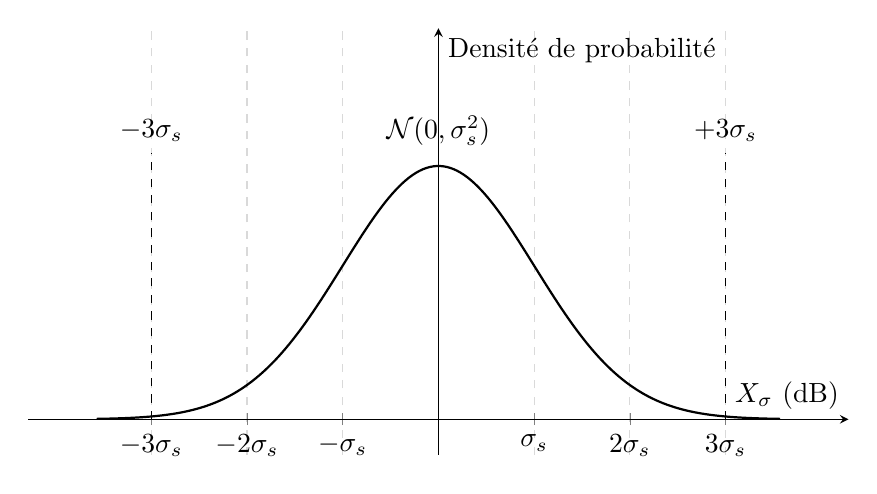
\begin{tikzpicture}
			\begin{axis}[
				width=12cm,
				height=7cm,
				domain=-25:25,
				samples=200,
				axis lines=middle,
				xlabel={$X_\sigma$ (dB)},
				ylabel={Densité de probabilité},
				ymin=0,
				ymax=0.08,
				xtick={-21,-14,-7,0,7,14,21},
				xticklabels={$-3\sigma_s$,$-2\sigma_s$,$-\sigma_s$,0,$\sigma_s$,$2\sigma_s$,$3\sigma_s$},
				ytick=\empty,
				enlargelimits=true,
				grid=both,
				grid style={dashed,gray!30}
				]
				
				% Gaussian curve (sigma = 7 dB)
				\addplot[thick] {1/(7*sqrt(2*pi)) * exp(-x^2/(2*7^2))};
				
				% Vertical lines for ±3σ
				\addplot[dashed] coordinates {(-21,0) (-21,0.06)};
				\addplot[dashed] coordinates {(21,0) (21,0.06)};
				
				\node at (axis cs:0,0.065) {$\mathcal{N}(0,\sigma_s^2)$};
				\node at (axis cs:21,0.065) {$+3\sigma_s$};
				\node at (axis cs:-21,0.065) {$-3\sigma_s$};
				
			\end{axis}
		\end{tikzpicture}
		\caption{Distribution gaussienne de l'ombrage avec $\sigma_s = 7$ dB.}
		\label{fig:shadowing_gaussian}
	\end{figure}
	
	\begin{figure}[H]
		\centering
		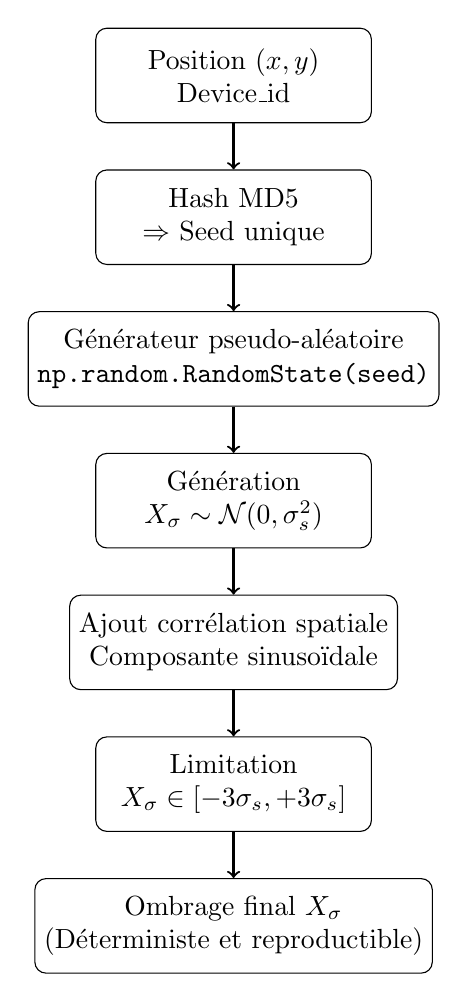
\begin{tikzpicture}[
			node distance=1.8cm,
			block/.style={rectangle, draw, rounded corners, align=center, minimum width=3.5cm, minimum height=1.2cm},
			arrow/.style={->, thick}
			]
			
			% Inputs
			\node[block] (input) {Position $(x,y)$ \\ Device\_id};
			
			% Hash
			\node[block, below of=input] (hash) {Hash MD5 \\ $\Rightarrow$ Seed unique};
			
			% RNG
			\node[block, below of=hash] (rng) {Générateur pseudo-aléatoire \\ \texttt{np.random.RandomState(seed)}};
			
			% Gaussian
			\node[block, below of=rng] (gauss) {Génération \\ $X_\sigma \sim \mathcal{N}(0,\sigma_s^2)$};
			
			% Spatial correlation
			\node[block, below of=gauss] (spatial) {Ajout corrélation spatiale \\ Composante sinusoïdale};
			
			% Clipping
			\node[block, below of=spatial] (clip) {Limitation \\ $X_\sigma \in [-3\sigma_s, +3\sigma_s]$};
			
			% Output
			\node[block, below of=clip] (output) {Ombrage final $X_\sigma$ \\ (Déterministe et reproductible)};
			
			% Arrows
			\draw[arrow] (input) -- (hash);
			\draw[arrow] (hash) -- (rng);
			\draw[arrow] (rng) -- (gauss);
			\draw[arrow] (gauss) -- (spatial);
			\draw[arrow] (spatial) -- (clip);
			\draw[arrow] (clip) -- (output);
			
		\end{tikzpicture}
		\caption{Architecture du modèle de l'ombrage déterministe}
		\label{fig:shadowing_model}
	\end{figure}
	
	La figure \ref{fig:shadowing_model} détaille le processus de génération de l'ombrage (\textit{shadowing}), garantissant la reproductibilité des expériences.
\end{itemize}

\subsection{Paramètres LR-FHSS implémentés}

Les paramètres de modulation suivent les spécifications RP002-1.0.5, avec les quatre débit de données supportés :

\begin{center}
	\begin{table}[H]
		\caption{Paramètres des débit de données (DR) utilisés}
		\centering
		\begin{tabular}{|c|r|c|r|}
			\hline
			\textbf{DR} & \textbf{BW (kHz)} & \textbf{CR} & \textbf{Débit (bps)} \\
			\hline
			DR8  & 137 & 1/3 & 162 \\
			DR9  & 137 & 2/3 & 325 \\
			DR10 & 336  & 1/3 & 162 \\
			DR11 & 336  & 2/3 & 325 \\
			\hline
		\end{tabular}
	\end{table}
\end{center}

Le temps d'antenne (ToA) est calculé selon la formule selon les equations \ref{eq:toa1} pour CR 1/3 et \ref{eq:toa2} pour CR 2/3.
La génération des séquences de saut de fréquence (FHS) repose sur un dictionnaire de 384 séquences produites par un registre à décalage à rétroaction linéaire (LFSR) de 9 bits \cite{lfsr}.

\subsection{Détection des collisions et évaluation du succès}

Deux fragments sont considérés en collision s'il y a chevauchement temporel et si leurs fréquences centrales sont suffisamment proches :

\begin{equation}
	|\Delta f| < 1.5 \times B_{inst}
	\label{eq:collision_freq}
\end{equation}

où \(\Delta f\) est l'écart en fréquence entre les deux fragments et \(B_{inst} = 488{,}28125\ Hz\) la bande passante instantanée d'un fragment. Le chevauchement spectral est calculé et une collision n'est significative que si le recouvrement dépasse 20\%. En l'absence de collision, le succès dépend de la marge de SNR. En cas de collision, l'évaluation se fait en tenant compte de la capacité de correction du FEC en fonction du DR.

\subsection{Métriques et reproductibilité}

Le simulateur calcule deux métriques temporelles : le ToA brut (somme des durées de tous les paquets) et le ToA net (temps effectif d’occupation du canal). Il évalue également la consommation énergétique engendrée par la transmission de ces paquets. D'autres métriques secondaires sont également calculées pour avoir une vue globale quantitative et qualitative de la simulation.  La reproductibilité est garantie par l'utilisation de graines déterministes pour le positionnement des nœuds et l'ombrage.

\subsection{Calcul de l'énergie par paquet}

La consommation énergétique de chaque transmission est calculée à partir du temps d'antenne (ToA) et de la puissance d'émission, en s'appuyant sur les profils de consommation mesurés sur des modules réels \cite{ullah2024_energy}. L'énergie consommée pour la transmission d'un paquet s'exprime par :

\begin{equation}
	E_{\text{TX}} = I_{\text{TX}}(P_{\text{TX}}) \times V \times ToA
	\label{eq:energie_tx}
\end{equation}

où \(I_{\text{TX}}(P_{\text{TX}})\) est le courant de transmission (en ampères) dépendant de la puissance d'émission \(P_{\text{TX}}\) (en dBm), \(V = 3,3\,\text{V}\) est la tension d'alimentation, et \(ToA\) est le temps d'antenne en secondes. Le courant de transmission \(I_{\text{TX}}(P_{\text{TX}})\) est obtenu par interpolation et extrapolation à partir des profils de consommation des modules SX1261 (Low Power PA) et SX1262 (High Power PA) \cite{semtech_1261_2}.

Cette approche, conforme aux caractérisations expérimentales de \cite{sanchez2024}, permet d'obtenir des estimations réalistes de l'énergie consommée par paquet en fonction des paramètres de transmission LR-FHSS.

\subsection{Validation expérimentale}

La crédibilité d'un simulateur repose sur sa capacité à reproduire fidèlement le comportement d'un système réel. Pour valider notre modèle, nous avons confronté ses prédictions à des mesures issues d'une série de mesures publiées dans la littérature \cite{lrfhss_comparaison}.

\subsubsection{Méthodologie de validation}

La validation a été réalisée en comparant les sorties de notre simulateur avec les données réelles publiées dans l'étude de Sanchez et al. \cite{sanchez_vital_2025_data}, qui fournit des mesures de PDR et de RSSI pour les quatre débits de données LR-FHSS à différentes distances.

Le protocole de validation est le suivant :
\begin{itemize}
	\item \textbf{Données d'entrée} : Pour chaque point de mesure réel, configuration du simulateur avec les paramètres correspondants (puissance 14 dBm, DR).
	
	\item \textbf{Paramètres de canal} : Exposant d'affaiblissement \(n=3,3\) et écart-type de l'ombrage \(\sigma_s = 7,0\ dB\), représentatifs d'un environnement urbain dense.
	
	\item \textbf{Exécution} : Simulations de 30 minutes avec 10 nœuds, générant environ 400 paquets par configuration.
\end{itemize}

\subsubsection{Analyse comparative par DR}

Les figures \ref{fig:dr8_validation} à \ref{fig:dr11_validation} présentent, pour chaque DR, la comparaison du PDR et du RSSI entre la simulation et les mesures réelles.

\begin{figure}[H]
	\centering
	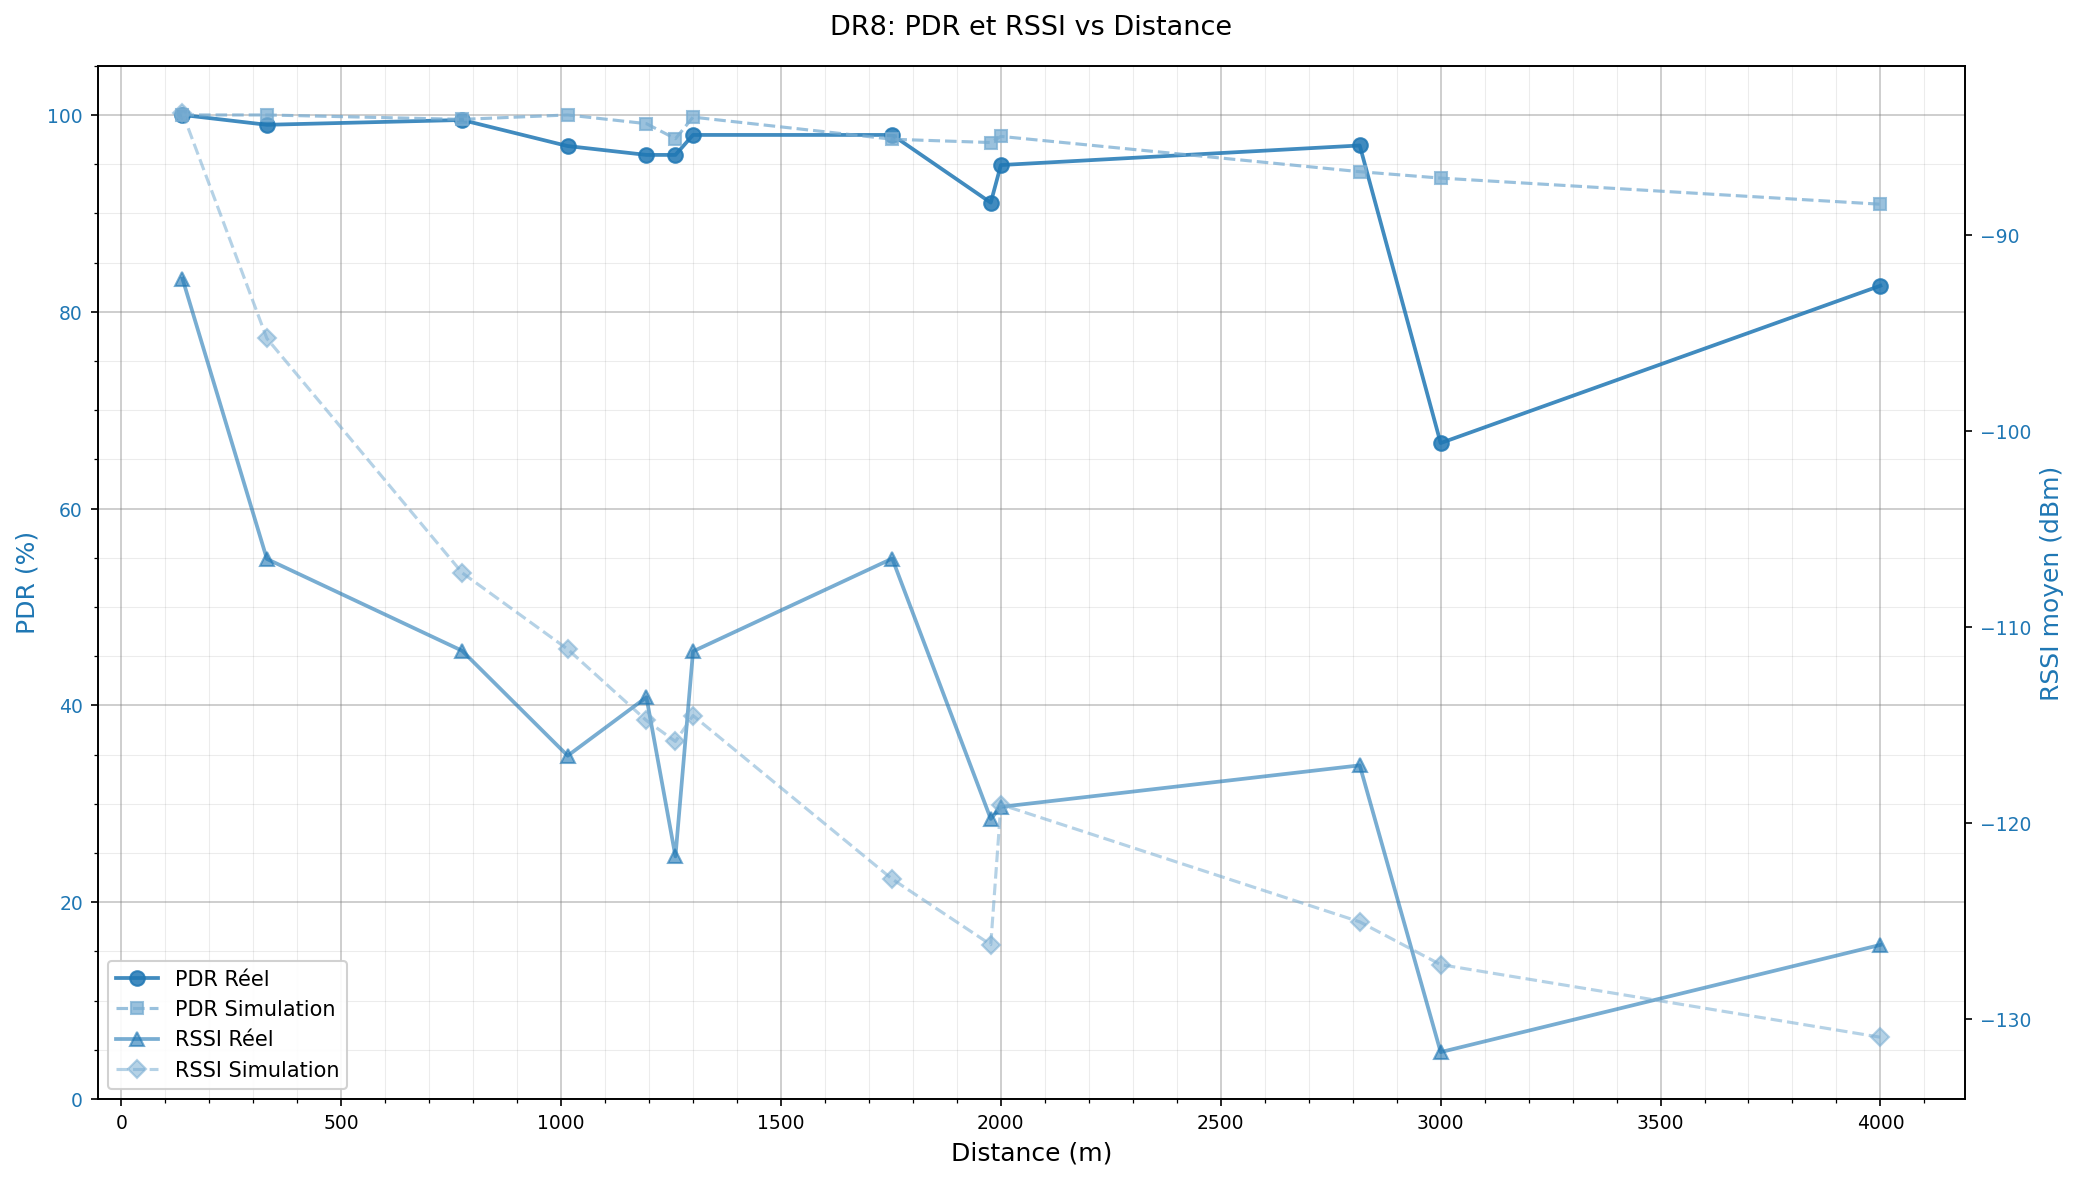
\includegraphics[width=0.8\textwidth]{images/validation/sim/dr8_pdr_rssi_vs_distance.png}
	\caption{Validation du modèle pour DR8 (CR=1/3, BW=137 kHz)}
	\label{fig:dr8_validation}
\end{figure}

Pour le DR8, les résultats montrent une bonne adéquation du modèle de RSSI, avec une erreur moyenne de 7,21 dB sur l'ensemble des distances. Le PDR simulée suit fidèlement la tendance réelle, avec une erreur quadratique moyenne de 10 \%.

\begin{figure}[H]
	\centering
	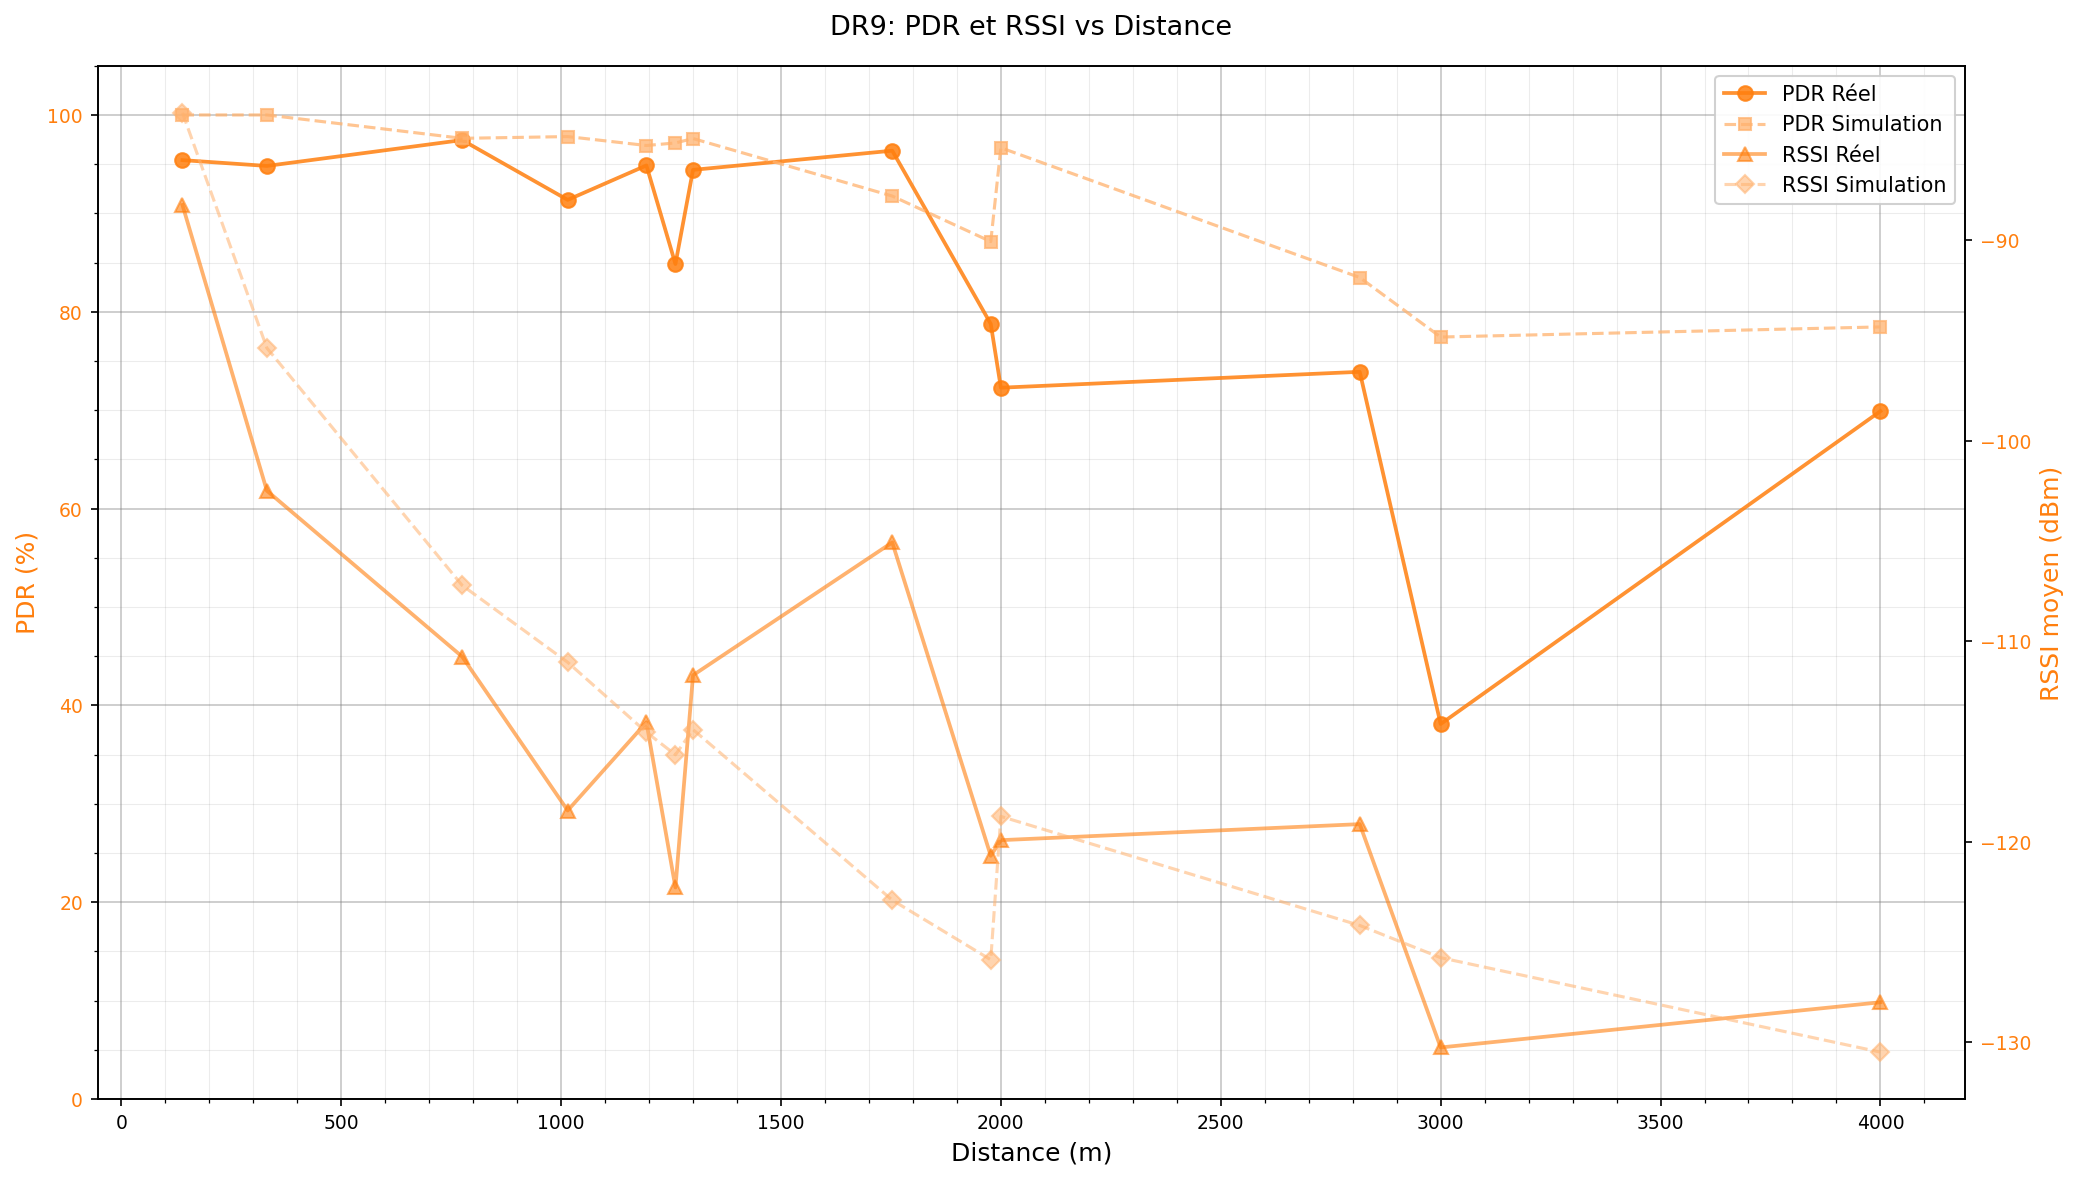
\includegraphics[width=0.8\textwidth]{images/validation/sim/dr9_pdr_rssi_vs_distance.png}
	\caption{Validation du modèle pour DR9 (CR=2/3, BW=137 kHz)}
	\label{fig:dr9_validation}
\end{figure}

Le DR9 montre une sensibilité accrue aux conditions de canal, ce qui se traduit par une décroissance plus rapide du PDR avec la distance. Le simulateur capture correctement cette tendance mais avec une erreur quadratique moyenne du PDR plus élevée de 21,40 \% et du RSSI de 6,84 dB.

\begin{figure}[H]
	\centering
	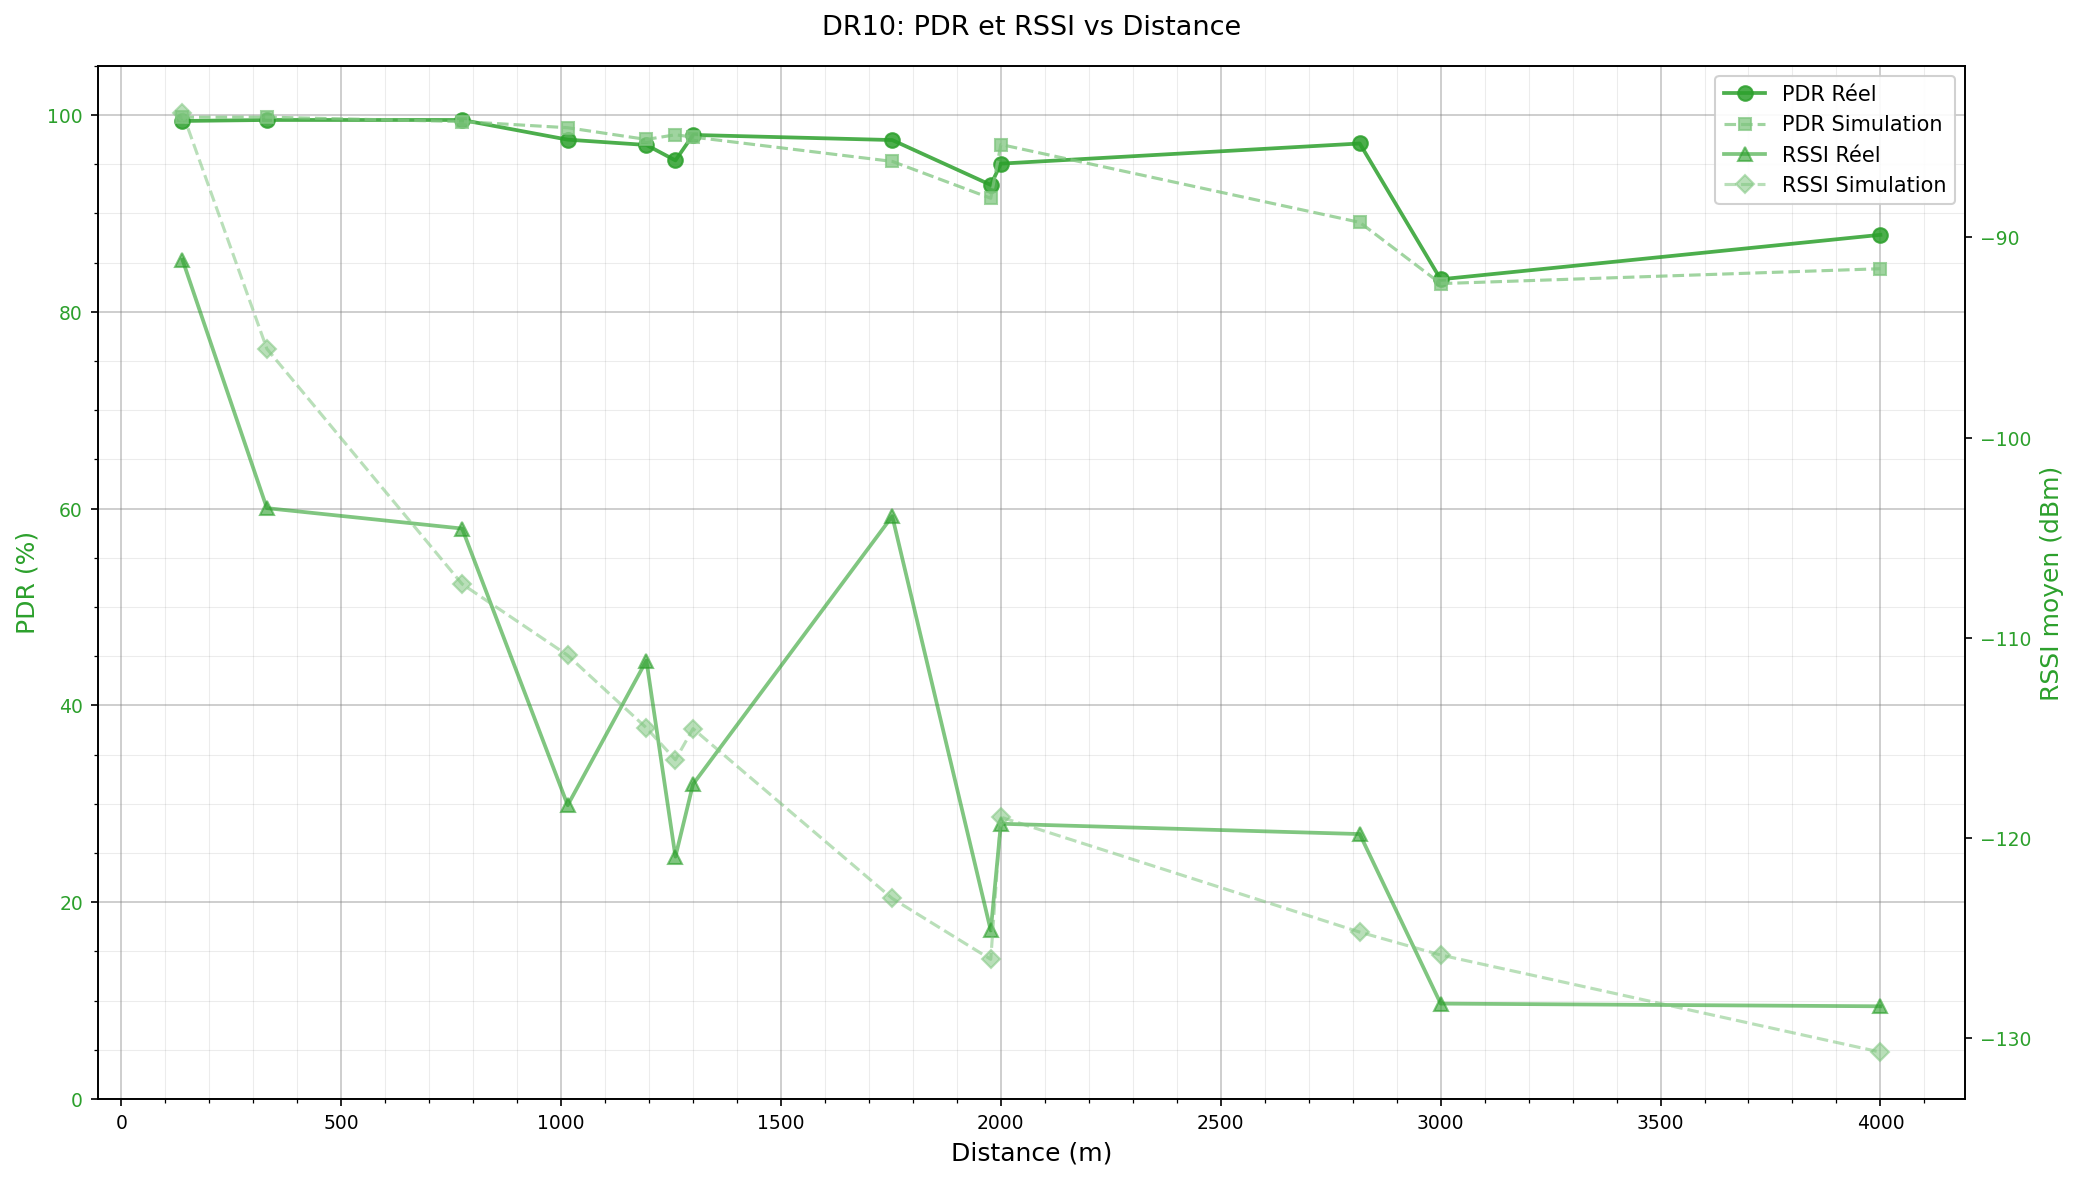
\includegraphics[width=0.8\textwidth]{images/validation/sim/dr10_pdr_rssi_vs_distance.png}
	\caption{Validation du modèle pour DR10 (CR=1/3, BW=336 kHz)}
	\label{fig:dr10_validation}
\end{figure}

Pour les DR à large bande, la validation est tout aussi concluante. Le DR10 maintient une PDR élevée (\(>90\%\)) jusqu'à 2000 m, et la simulation reproduit cette performance avec une grande fidélité. L'erreur quadratique moyenne pour le PDR est de 5,11 \% et pour RSSI 5,92 dB, la meilleure corrélation obtenue.

\begin{figure}[H]
	\centering
	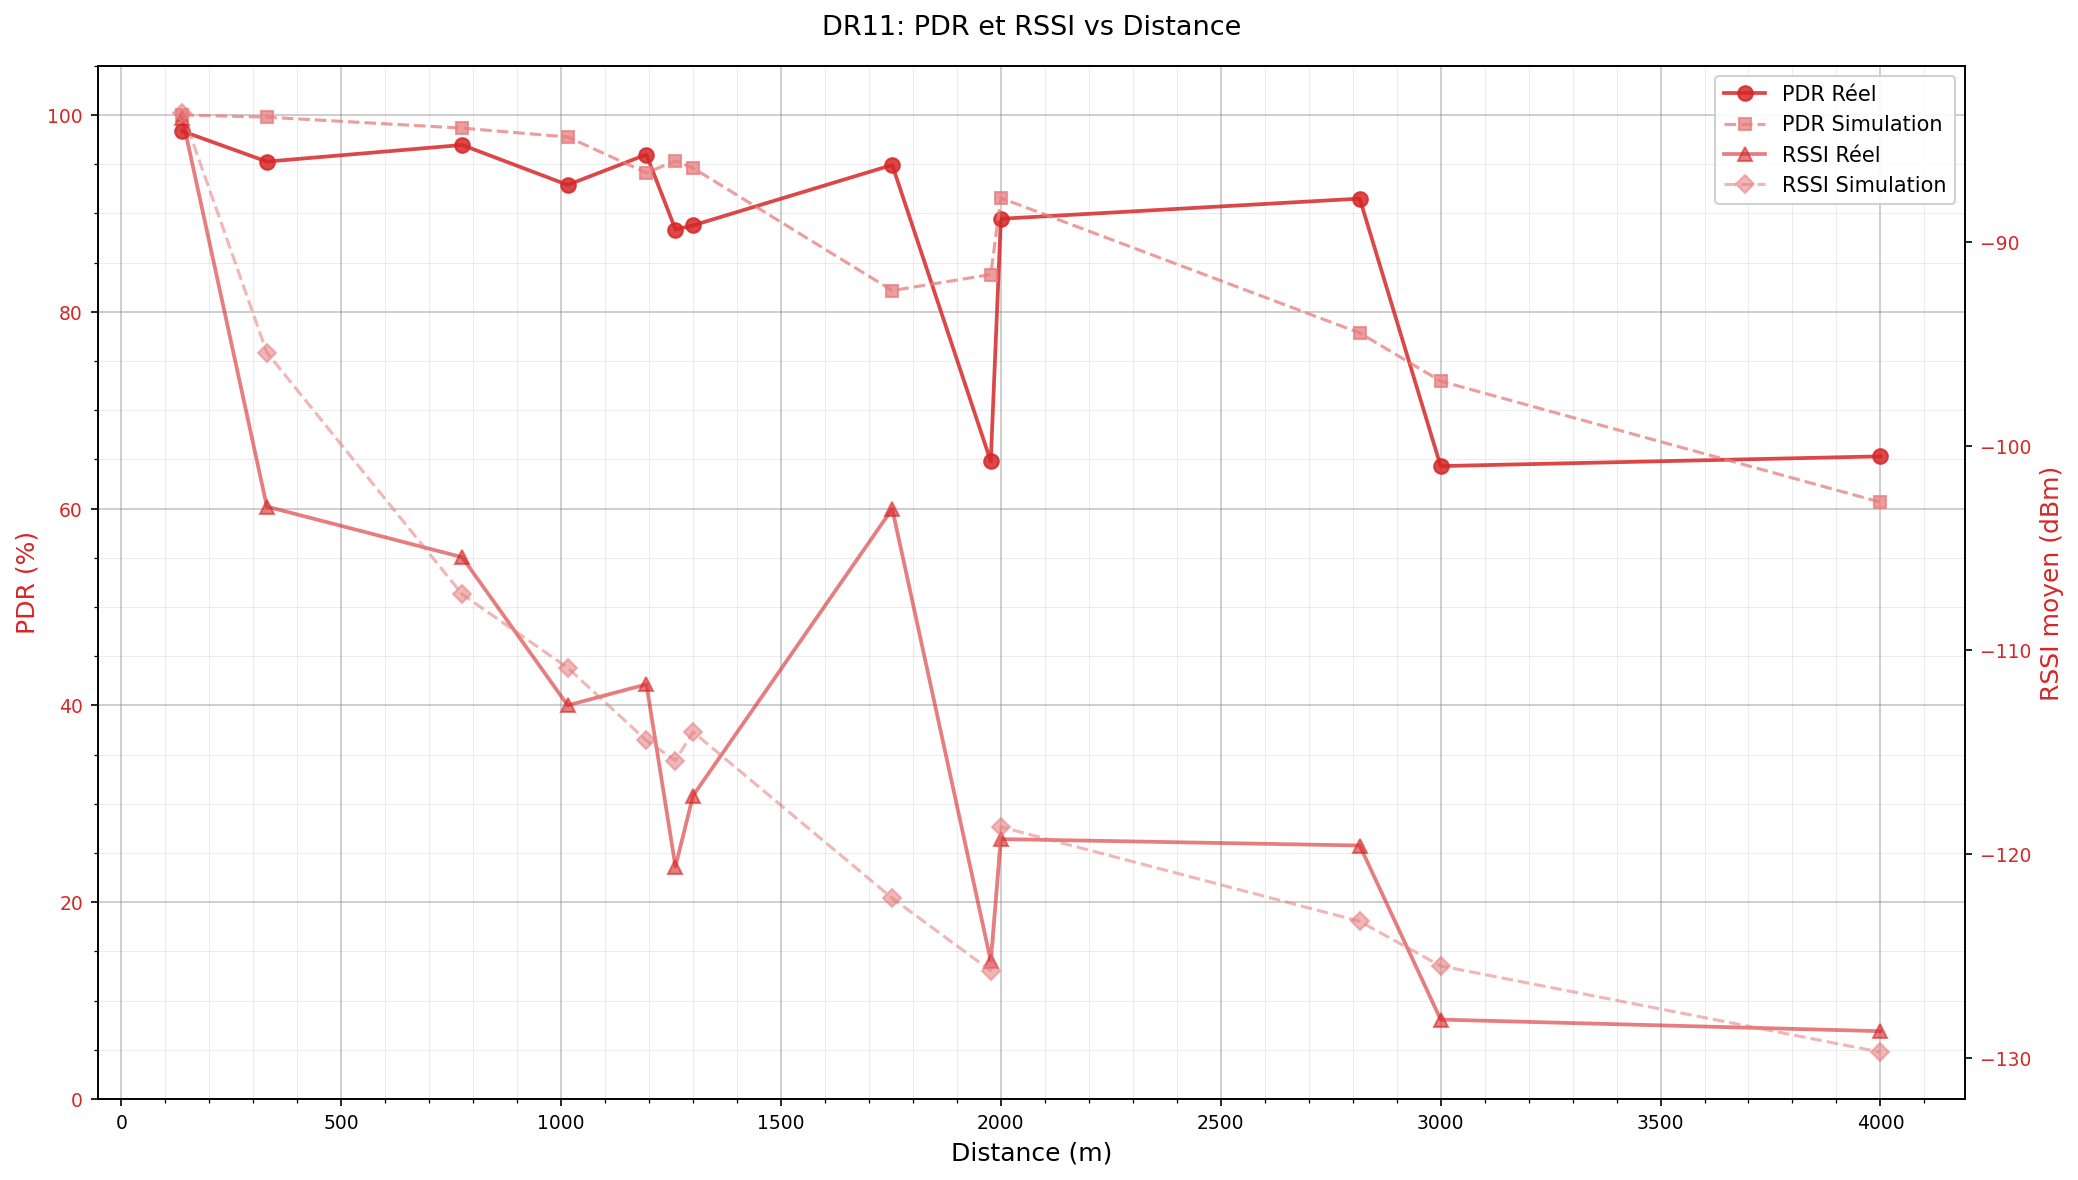
\includegraphics[width=0.8\textwidth]{images/validation/sim/dr11_pdr_rssi_vs_distance.png}
	\caption{Validation du modèle pour DR11 (CR=2/3, BW=336 kHz)}
	\label{fig:dr11_validation}
\end{figure}

Pour le DR11, on constate que le PDR chuter rapidement à partir de 1500 m. La simulation reproduit cette chute avec une erreur quadratique moyenne du PDR de 11,16 \% et pour le RSSI de 6,28 dB.

\newpage
\subsubsection{Analyse globale et quantification des erreurs}

La figure \ref{fig:pdr_global_validation} synthétise les performances de PDR pour l'ensemble des DR.

\begin{figure}[H]
	\centering
	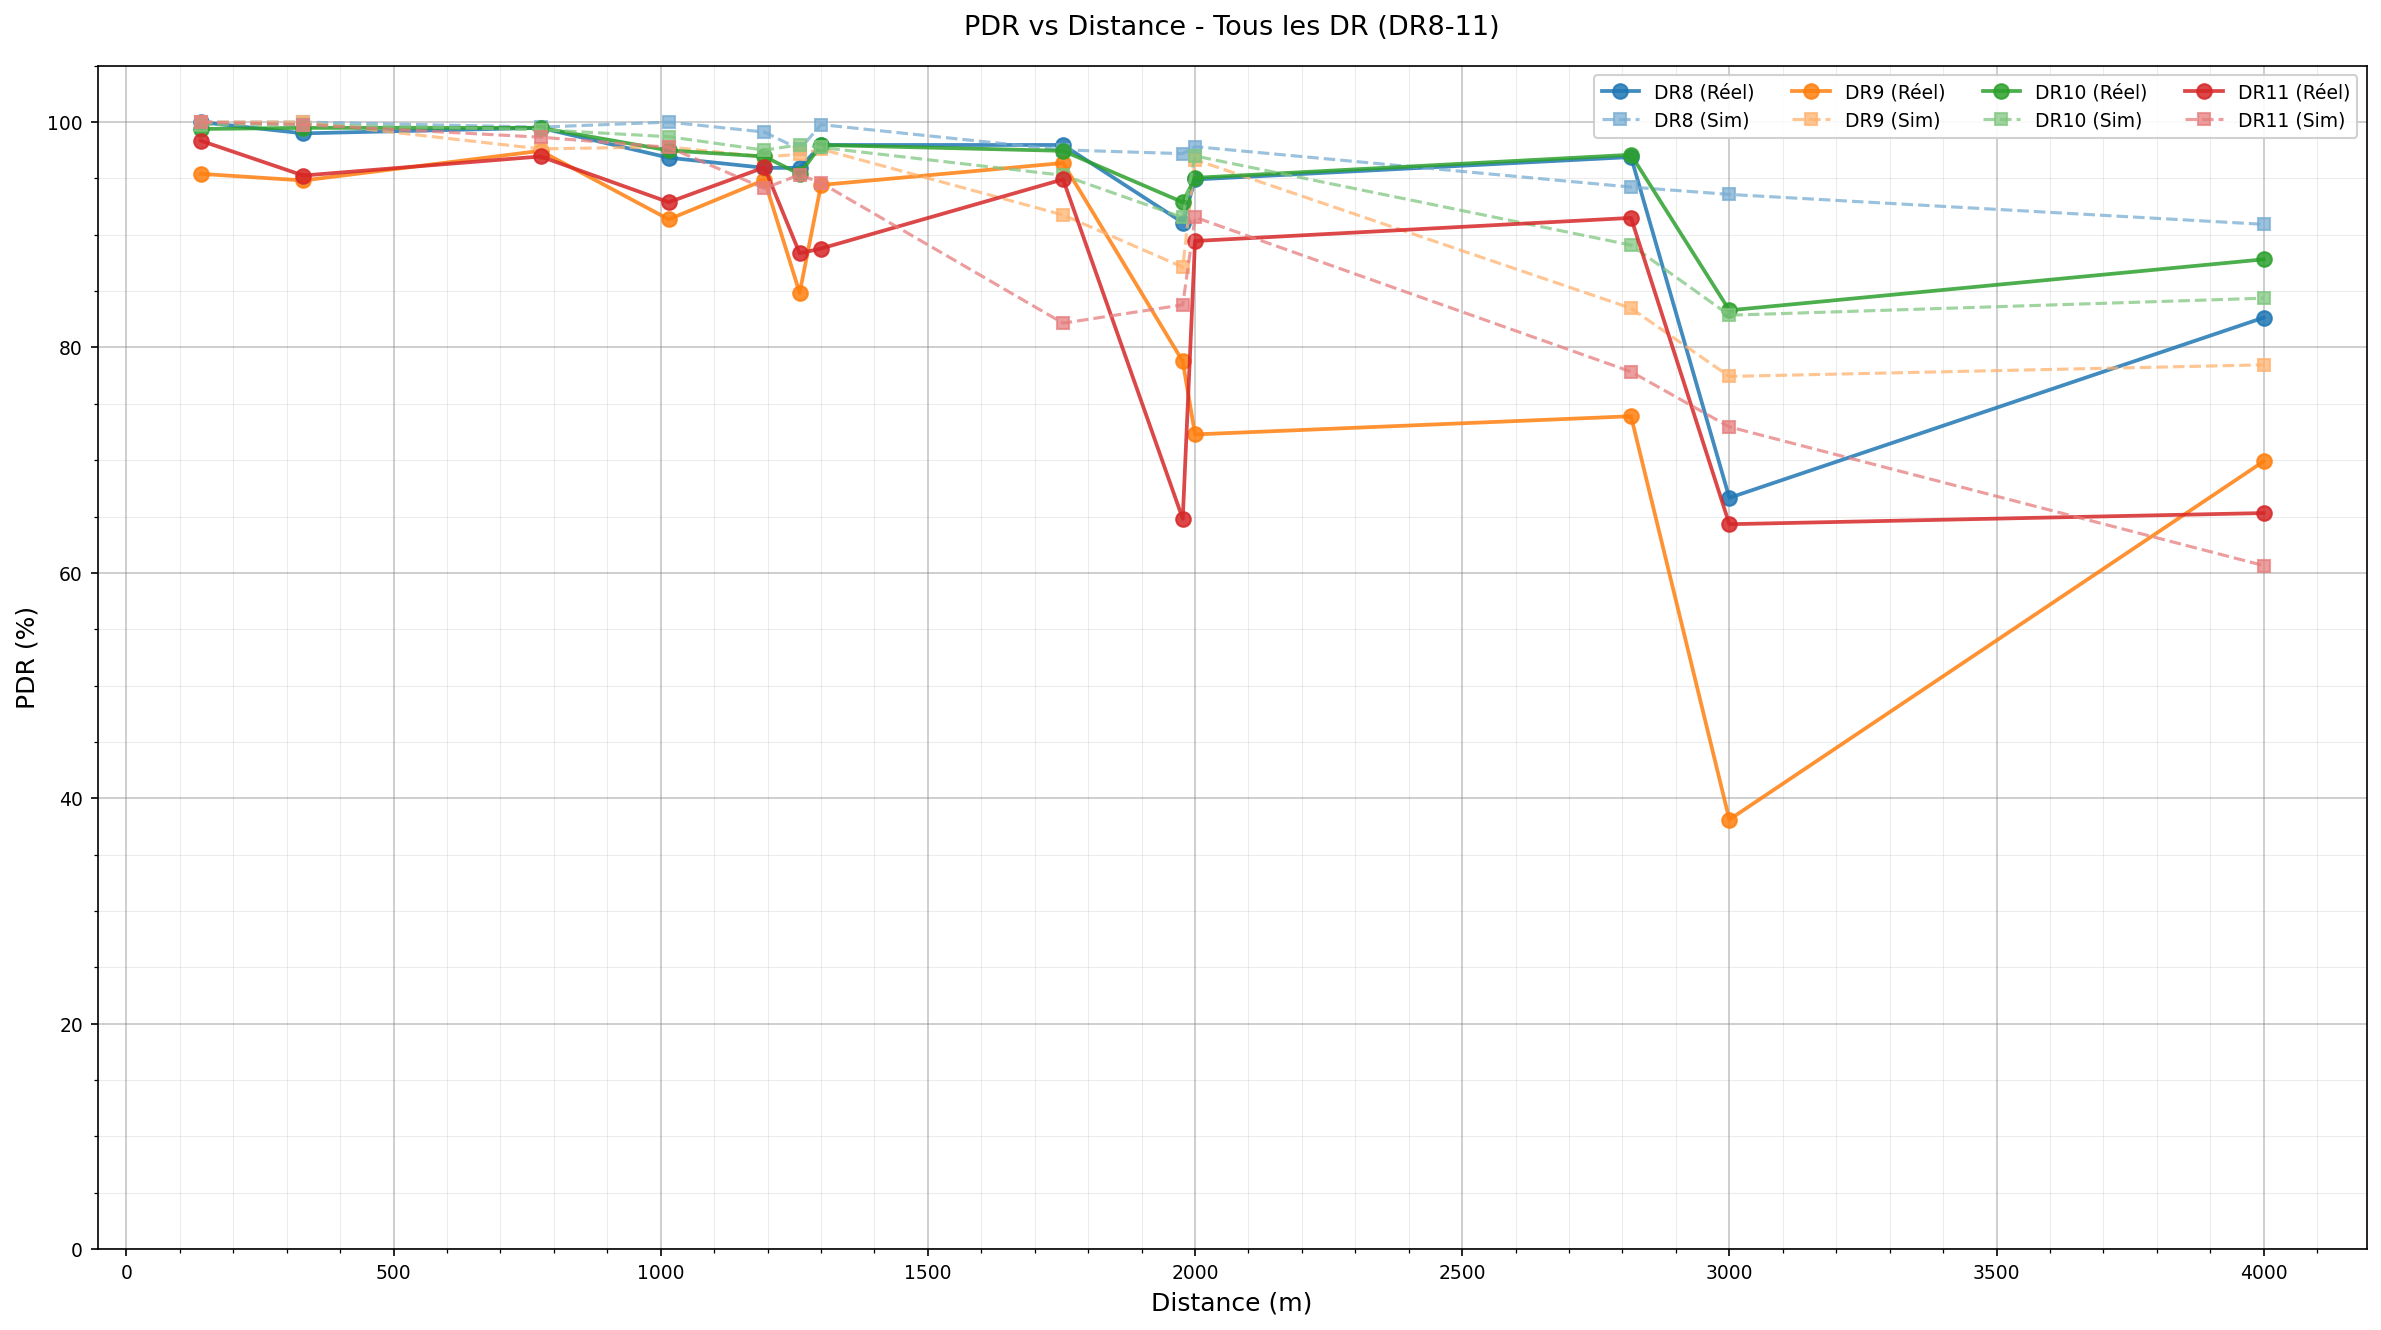
\includegraphics[width=0.9\textwidth]{images/validation/sim/all_dr_pdr_vs_distance.png}
	\caption{Comparaison globale du PDR : simulation et données mesurées}
	\label{fig:pdr_global_validation}
\end{figure}

Les résultats montrent une excellente corrélation globale. Le simulateur parvient à reproduire fidèlement :
\begin{itemize}
	\item La hiérarchie des performances entre les DR
	\item La forme caractéristique des courbes de PDR
\end{itemize}

La figure \ref{fig:rssi_global_validation} montre la comparaison pour le RSSI entre la simulation et les données mesurées.

\begin{figure}[H]
	\centering
	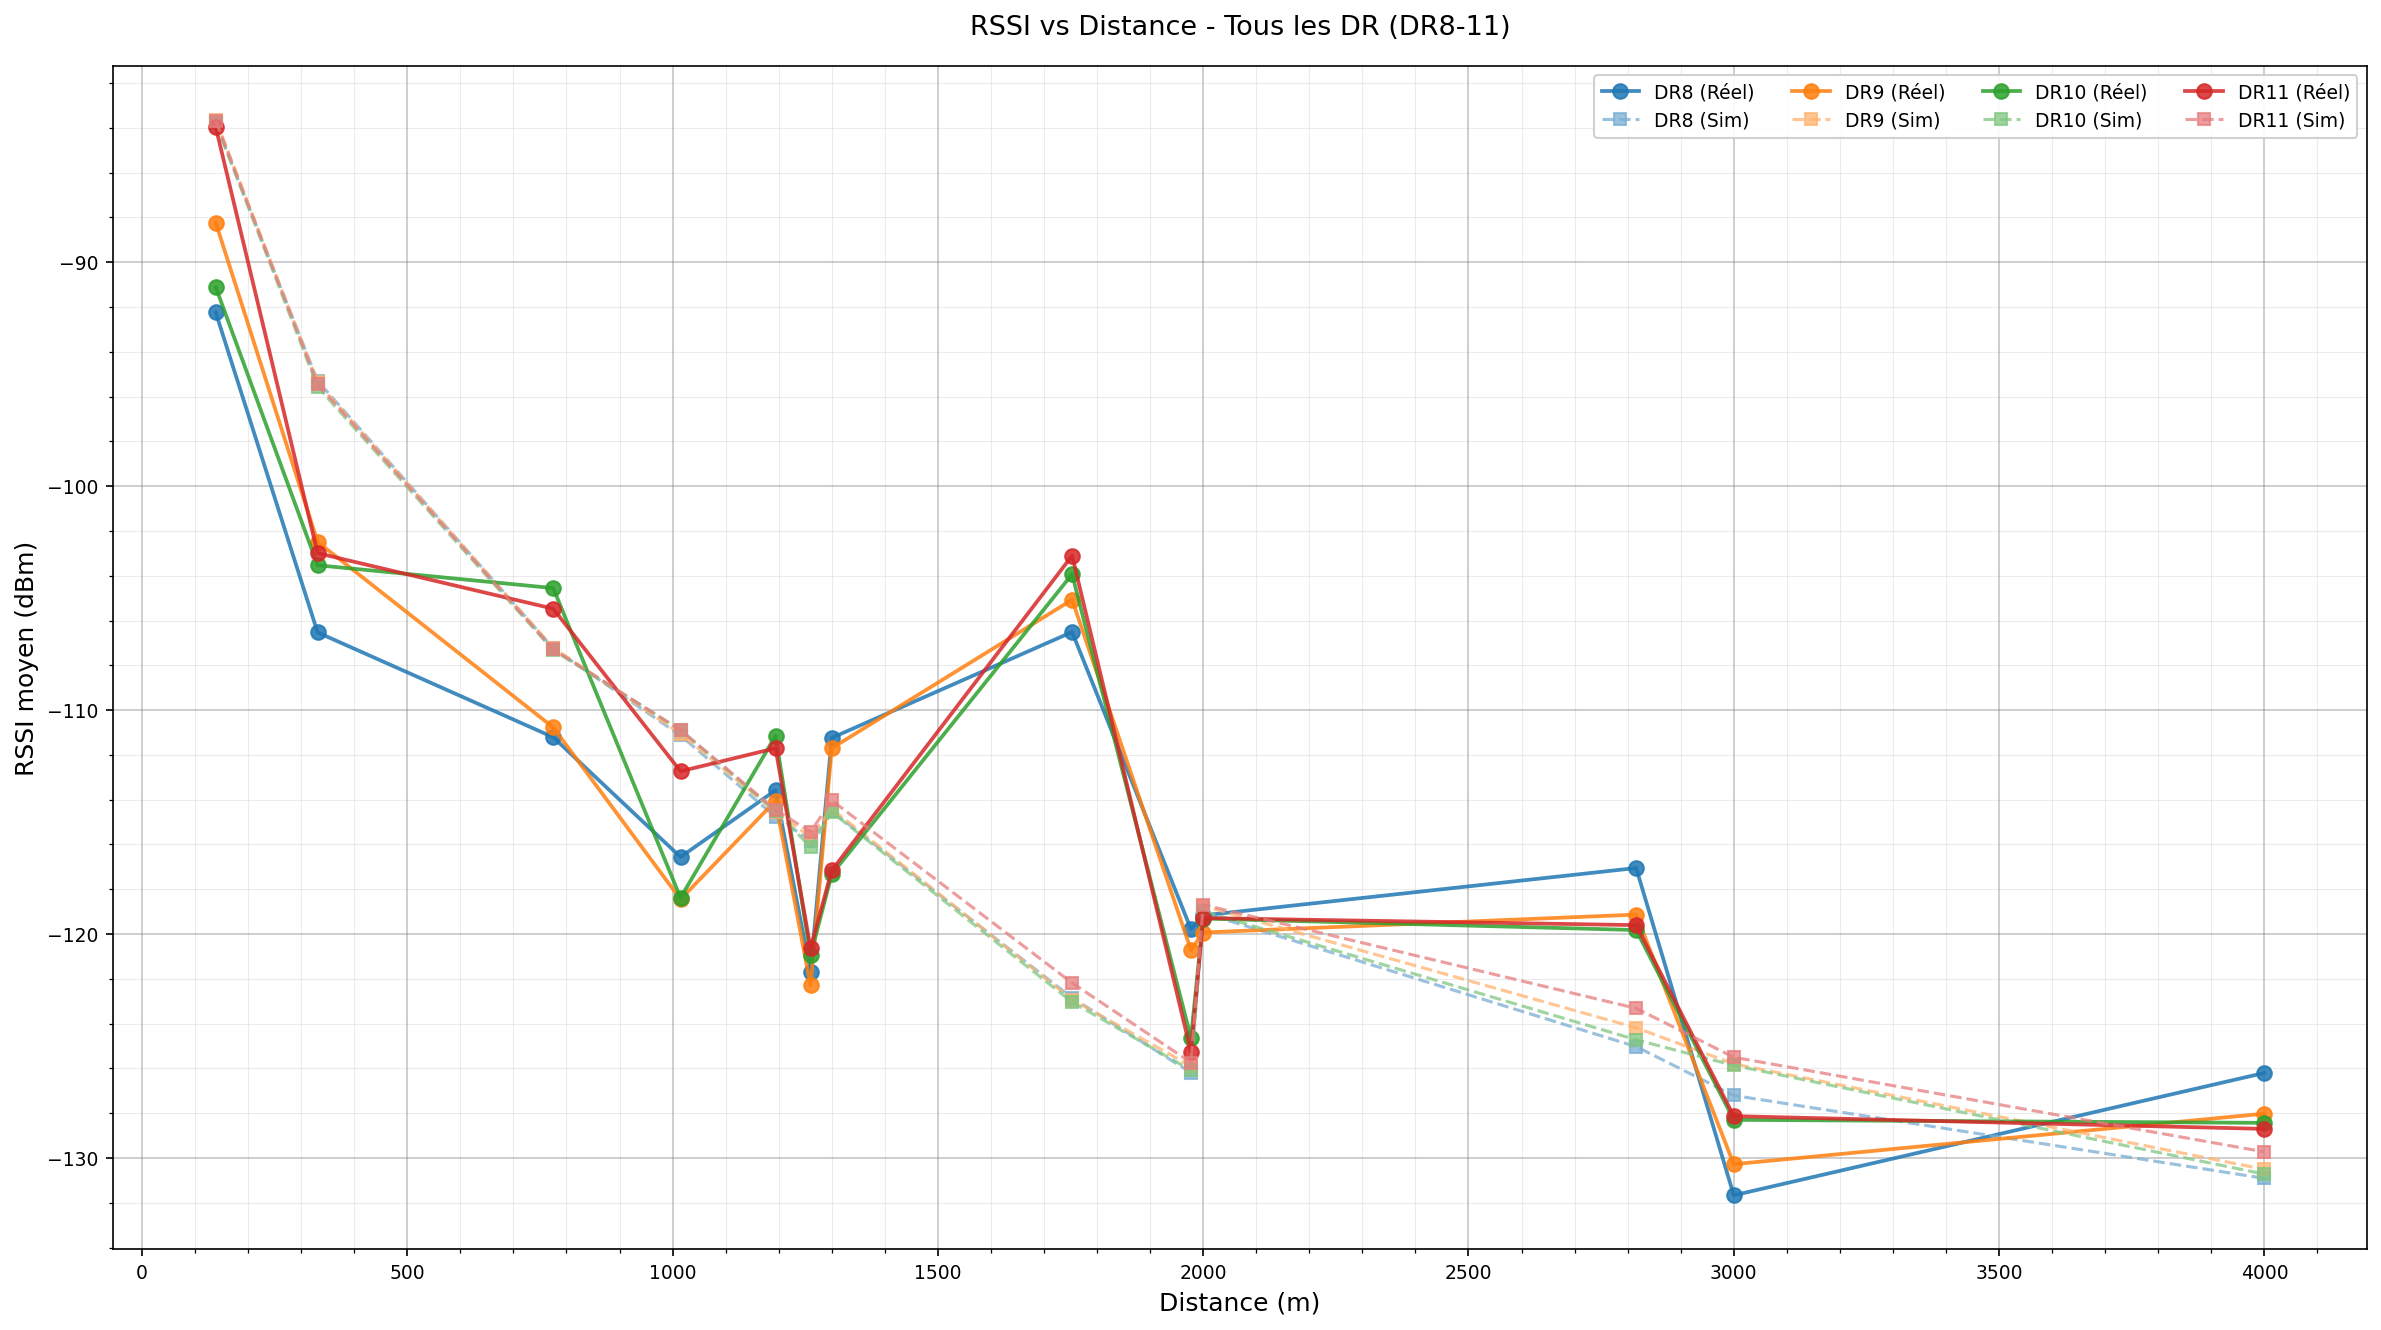
\includegraphics[width=0.9\textwidth]{images/validation/sim/all_dr_rssi_vs_distance.png}
	\caption{Comparaison globale du RSSI moyen}
	\label{fig:rssi_global_validation}
\end{figure}

L'adéquation du modèle de propagation est ici correcte. La simulation prédit le RSSI moyen avec une erreur moyenne de 6,56 dB pour l'ensemble des points de mesure, validant :
\begin{itemize}
	\item Le choix du modèle log-distance avec un exposant \(n=3,3\)
	\item La calibration de la perte de référence à 125 dB à 1 km
	\item Le modèle d'ombrage (\textit{shadowing}) déterministe basé sur la position\\
\end{itemize}

Pour la quantification rigoureuse  de la performance de notre simulateur, nous avons calculé l'erreur quadratique moyenne (RMSE) pour le PDR et le RSSI à l'aide de ces formules :

\begin{equation}
	\text{RMSE}_{\text{PDR}} \; [\%] = \sqrt{\frac{1}{N} \sum_{i=1}^{N} \left( \text{PDR}_{\text{réel},i} - \text{PDR}_{\text{sim},i} \right)^2} \times 100
	\label{eq:rmse_pdr}
\end{equation}

\begin{equation}
	\text{RMSE}_{\text{RSSI}} \; [\text{dB}] = \sqrt{\frac{1}{N} \sum_{i=1}^{N} \left( \text{RSSI}_{\text{réel},i} - \text{RSSI}_{\text{sim},i} \right)^2}
	\label{eq:rmse_rssi}
\end{equation}

où \(N\) est le nombre de points de mesure, \(\text{PDR}_{\text{réel},i}\) et \(\text{PDR}_{\text{sim},i}\) sont respectivement les PDR réelle et simulée au point \(i\), et \(\text{RSSI}_{\text{réel},i}\) et \(\text{RSSI}_{\text{sim},i}\) les RSSI correspondants.

Le tableau suivant fait une synthèse de ces erreurs pour chaque DR.

\begin{table}[H]
	\centering
	\caption{Erreurs quadratiques moyennes (RMSE) entre la simulation et les données réelles}
	\label{tab:validation_errors}
	\begin{tabular}{|c|c|c|}
		\hline
		\textbf{DR} & \textbf{RMSE PDR (\%)} & \textbf{RMSE RSSI (dB)} \\
		\hline
		DR8  & 10,69 & 7,21 \\
		DR9  & 21,40 & 6,84 \\
		DR10 & 5,11  & 5,92 \\
		DR11 & 11,38 & 6,28 \\
		\hline
		\textbf{Moyenne} & \textbf{12,14} & \textbf{6,56} \\
		\hline
	\end{tabular}
\end{table}

Après validation de ce simulateur, nous passons maintenant à l'évaluation de notre solution à l'aide de ce dernier.

\section{Méthodologie d'évaluation}
\label{sec:methodo-eval}
Cette sous-section détaille la méthodologie adoptée pour évaluer les performances de l’agent DDQN. Elle présente d’abord le protocole de simulation utilisé pour reproduire des scénarios réalistes, puis définit les métriques de performance retenues pour analyser la fiabilité, l’efficacité énergétique et l’adaptativité des transmissions

\subsection{Protocole}
\label{subsec:protocole-eval}

Pour garantir la reproductibilité et la pertinence de nos résultats, nous avons mis en place un protocole d'évaluation rigoureux :

\begin{enumerate}
	\item \textbf{Points de comparaison} : Nous utilisons les 13 distances du fichier de validation \cite{sanchez_vital_2025_data}, couvrant une plage de 139 m à 4000 m.
	\item \textbf{Configurations testées} :
	\begin{itemize}
		\item \textbf{Simulation standard} : Pour chaque distance et chaque DR, nous exécutons une simulation de 30 minutes avec 10 nœuds, paramétrée avec les caractéristiques physiques du DR et une puissance d'émission fixe de 14 dBm.
		\item \textbf{Simulation avec DDQN} : Pour chaque distance, nous exécutons une simulation où l'agent DDQN sélectionne dynamiquement le DR et la puissance pour chaque transmission.
	\end{itemize}
	\item \textbf{Métriques collectées} : Pour chaque simulation, nous enregistrons le PDR global, la distribution des choix de DR et de puissance, et la consommation énergétique par transmission.
	\item \textbf{Reproductibilité} : Pour chacune de ces simulations, nous avons les mêmes conditions : mêmes positions, même ombrage et même évaluation grâce à une \textit{seed} globale que nous pouvons faire varier.
\end{enumerate}

\subsection{Métriques de performance}
\label{subsec:metriques-eval}

Les performances sont évaluées selon trois axes :

\begin{itemize}
	\item \textbf{La fiabilité} : \(\text{PDR} = \frac{\text{Nombre de paquets reçus avec succès}}{\text{Nombre total de paquets émis}}\)
	\item \textbf{L'efficacité énergétique} : \(E_{\text{tx}} = \text{Énergie consommée par transmission} \ [\text{mJ}]\)
	\item \textbf{L'adaptativité} : Analysée à travers la distribution des choix de DR et de puissance en fonction de la distance.
\end{itemize}

\section{Résultats et analyse comparative}
\label{sec:resultats-analyse}
Cette section présente les résultats obtenus lors des simulations et analyse de manière comparative les performances entre la configuration statique (standard) et l’agent DDQN. Les évaluations sont effectuées globalement, puis détaillées selon les distances, le PDR, le débit, la puissance d’émission et la consommation énergétique.

\subsection{Analyse globale des performances}

La figure \ref{fig:pdr-comparison} présente une comparaison globale du PDR entre la simulation standard et la simulation avec DDQN.

\begin{figure}[H]
	\centering
	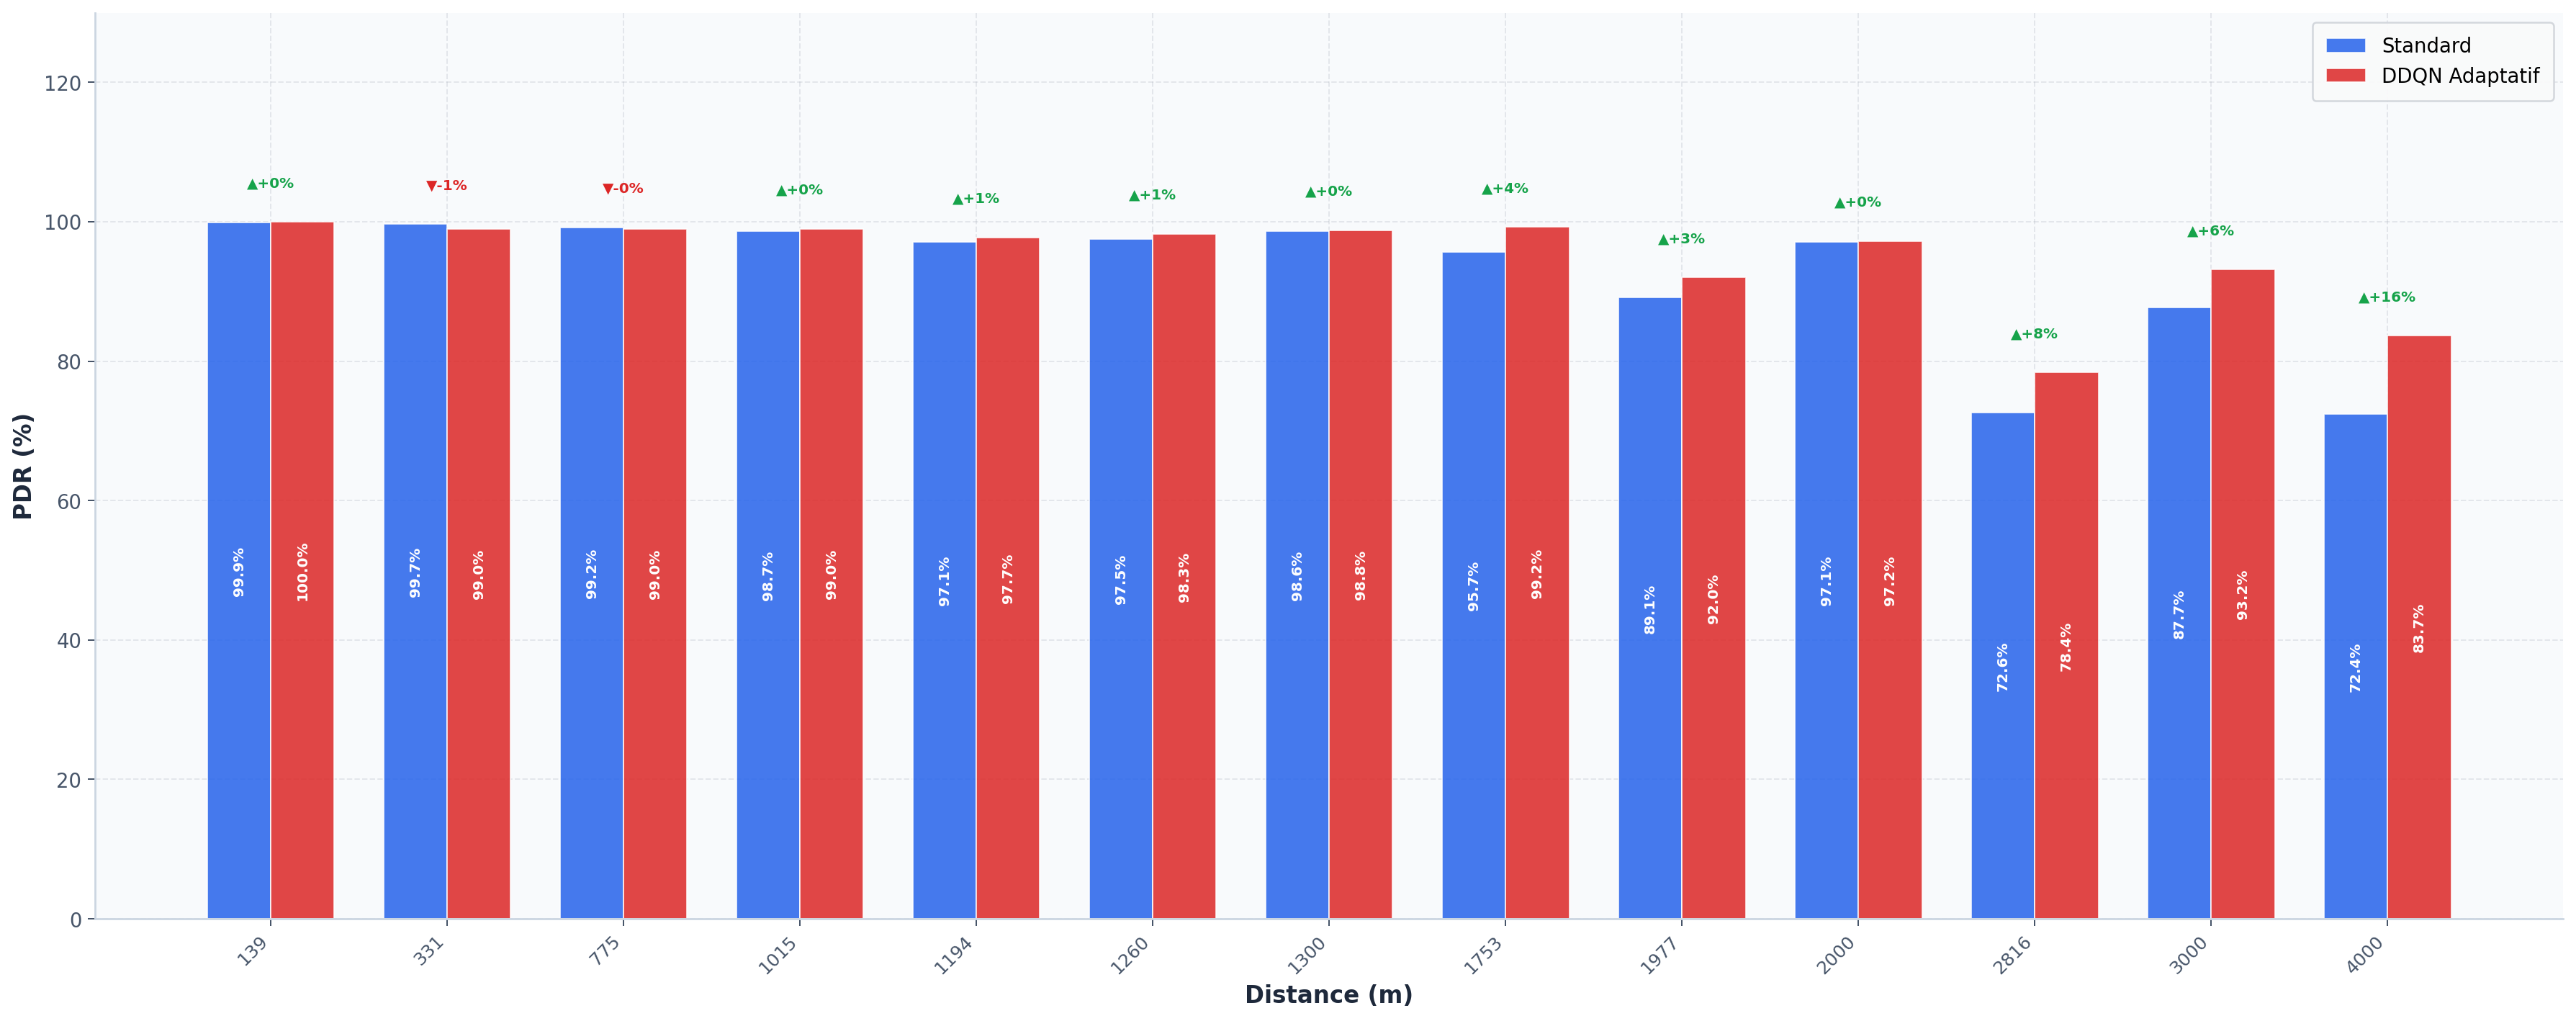
\includegraphics[width=1\textwidth]{images/validation/ddqn/pdr_by_distance.png}
	\caption{Comparaison du PDR entre simulation standard et agent DDQN}
	\label{fig:pdr-comparison}
\end{figure}

L'agent DDQN maintient un PDR systématiquement supérieur, particulièrement visible aux distances moyennes et longues : à 1753 m (99,2\% contre 95,7\%), à 2816 m (78,4\% contre 72,6\%), et à 4000 m (83,7\% contre 72,4\%, soit un gain absolu de 11,3 points et une amélioration relative de 15,6\%).

\subsection{Analyse de la stratégie d'adaptation du DDQN}

La figure \ref{fig:ddqn-dr-choices} illustre la distribution des choix de DR effectués par l'agent DDQN en fonction de la distance et la figure \ref{fig:ddqn-debit} l'évolution du débit découlant du choix du DR.

\begin{figure}[H]
	\centering
	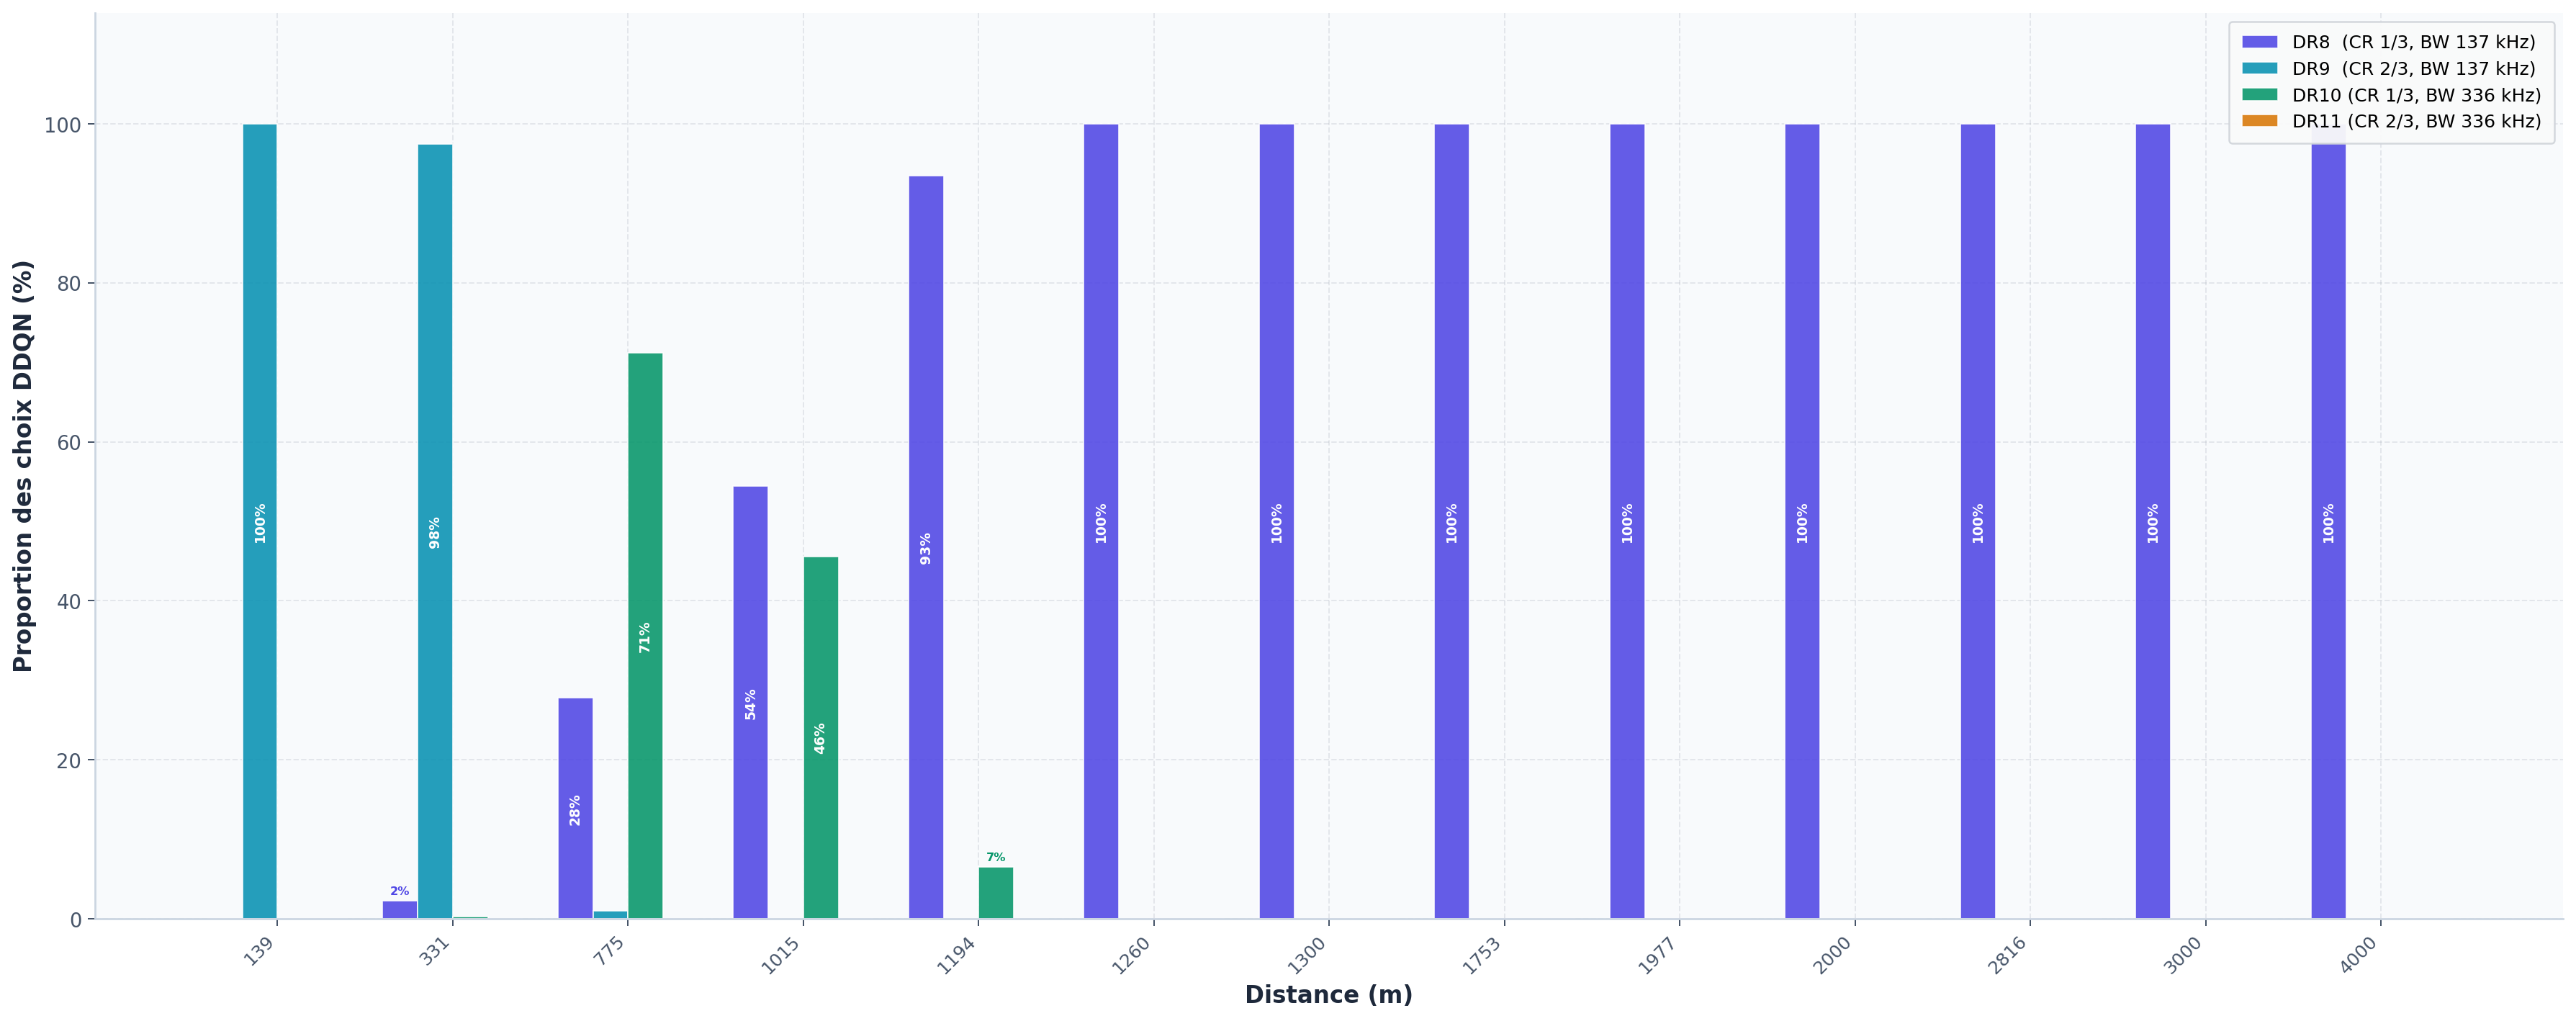
\includegraphics[width=1\textwidth]{images/validation/ddqn/ddqn_dr_choices.png}
	\caption{Distribution des DR choisis par l'agent DDQN en fonction de la distance}
	\label{fig:ddqn-dr-choices}
\end{figure}

\begin{figure}[H]
	\centering
	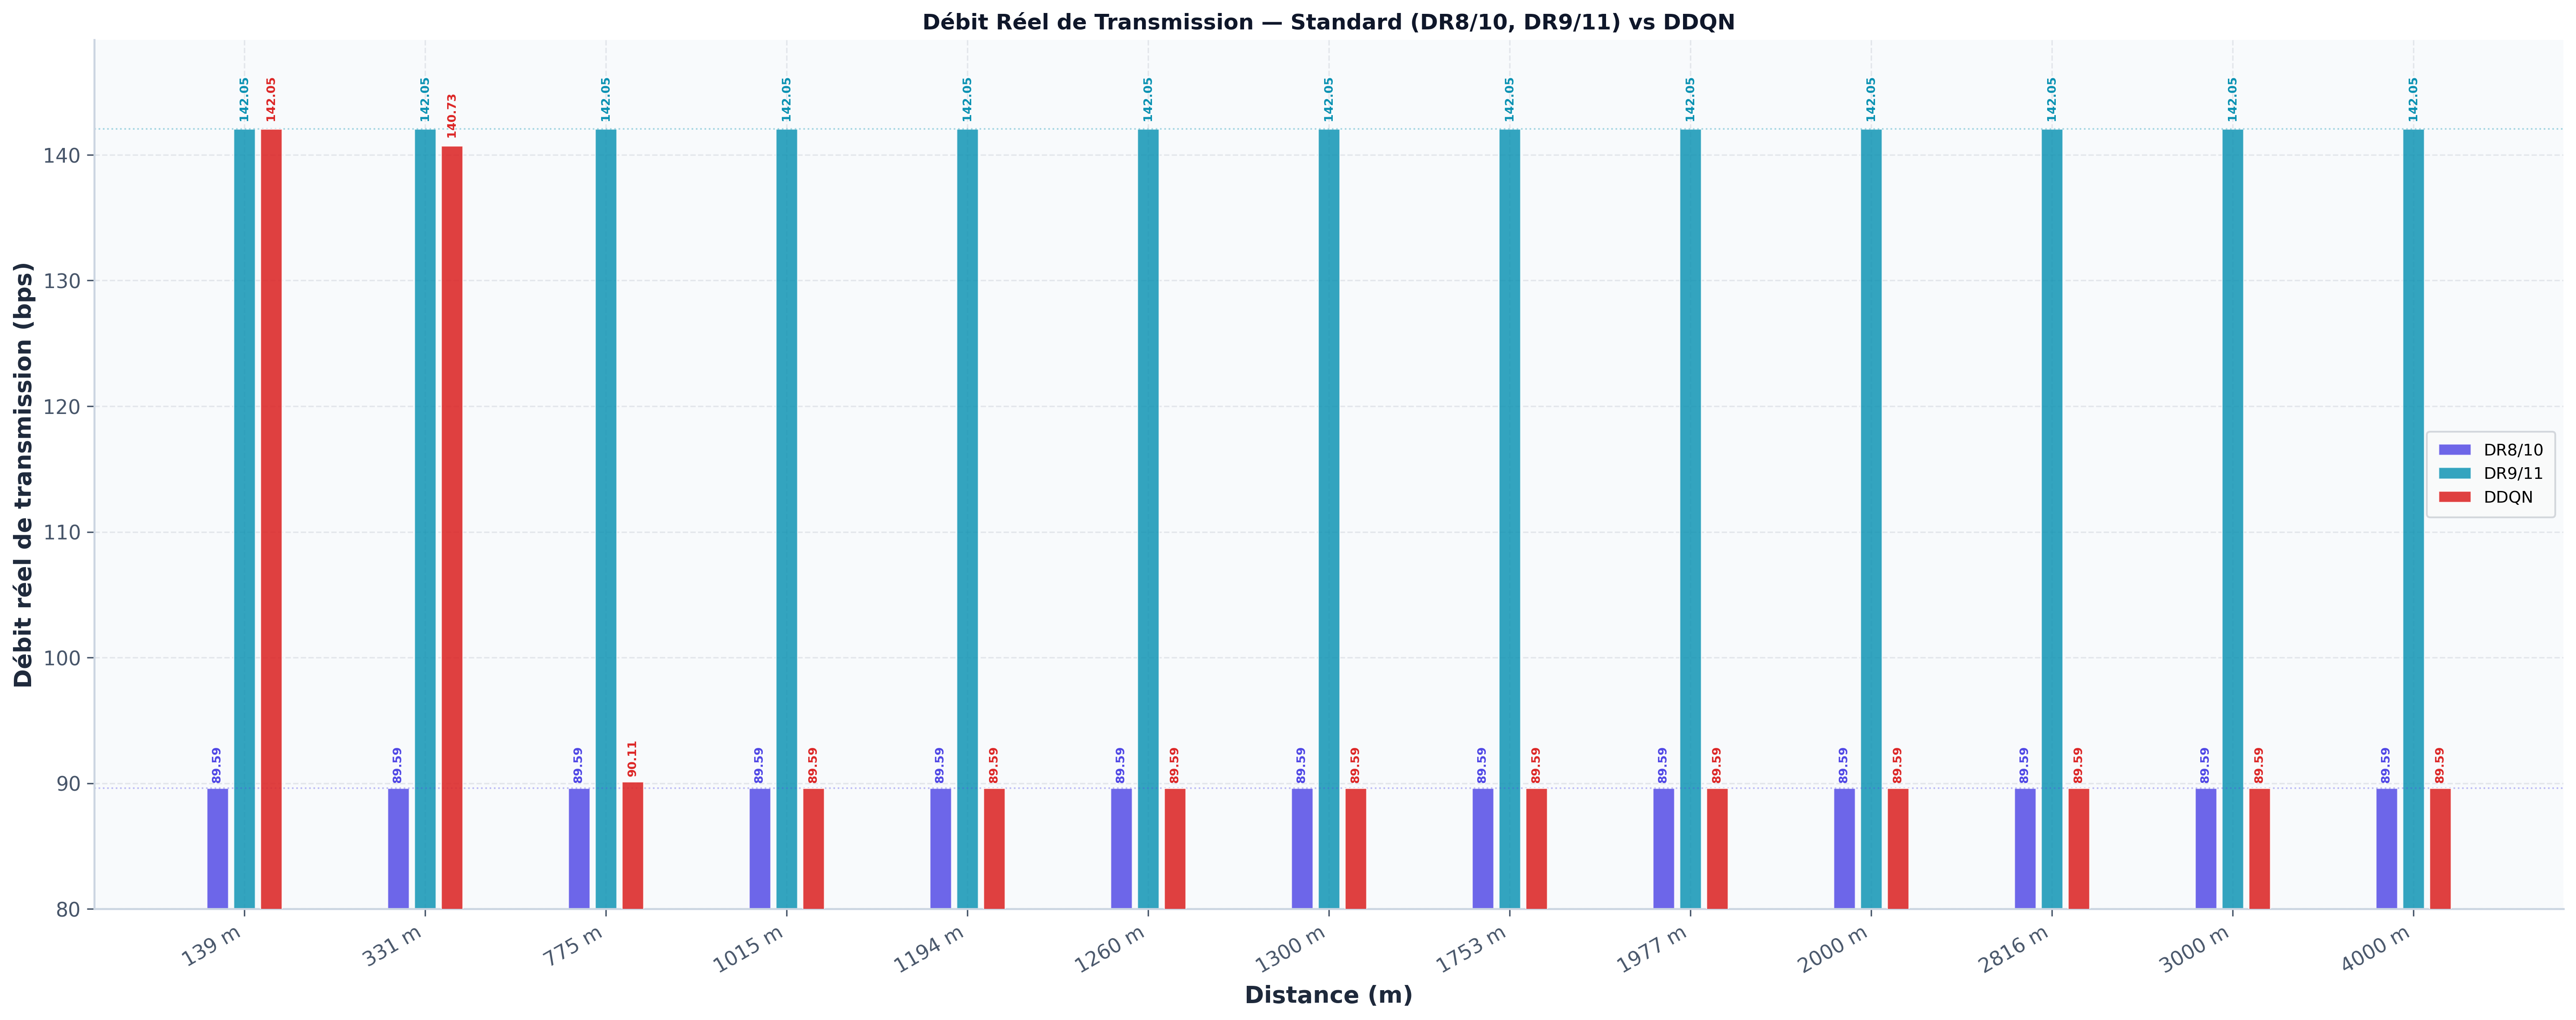
\includegraphics[width=1\textwidth]{images/validation/ddqn/debit_brut.png}
	\caption{Évolution du débit résultant du choix de DR}
	\label{fig:ddqn-debit}
\end{figure}

La politique d'adaptation est claire et progressive :
\begin{itemize}
	\item À courte distance (139 m), le DDQN atteint son \textbf{débit maximal} de 142,05 bps. Cela s'explique par l'utilisation exclusive des DR9/11 (100\%), qui permettent un débit plus élevé.
	
	\item À  331 m, le DDQN reste proche du débit  maximal (140,73 bps), grâce à une utilisation encore majoritaire de DR9/11 (98 \%) et DR8/10 (2 \%).
	
	\item À moyenne distance (775 m), le débit du DDQN chute à 90,11 bps. Cela correspond à une transition vers les DR8/10 (99\%) et DR9/11 (1\%), utilisé pour maintenir la fiabilité des transmissions à plus longue distance.
	
	\item Sur les longues distances (1015–4000 m), le DDQN utilise exclusivement le DR8/10 (100\%), ce qui explique le débit réduit (89,59 bps). Cette stratégie illustre la capacité de l'agent DDQN à adapter dynamiquement le DR en fonction de la distance pour maximiser la fiabilité au détriment d'un débit élevé.
	
	\item En comparaison, la moyenne entre DR8/10 et DR9/11 est de 115,82 bps, mais le DDQN peut dépasser cette moyenne à courte distance grâce à la sélection intelligente du DR le plus performant.
\end{itemize}

Cette stratégie est alignée avec la théorie des communications : utiliser les DR les plus efficaces (haut débit) quand le canal le permet, et basculer vers des configurations robustes quand les conditions se dégradent.

\subsection{Analyse comparative détaillée par DR}

Pour valider la stratégie d'adaptation de l'agent DDQN, nous avons comparé ses performances pour chaque configuration de DR (DR8 à DR11). Les figures \ref{fig:dr8-pdr} à \ref{fig:dr11-rssi} présentent la comparaison des PDR et des RSSI pour chaque DR.

\newpage
\begin{itemize}
	\item \textbf{Analyse pour DR8 (CR 1/3, BW 137 kHz)}
	
	\begin{figure}[H]
		\centering
		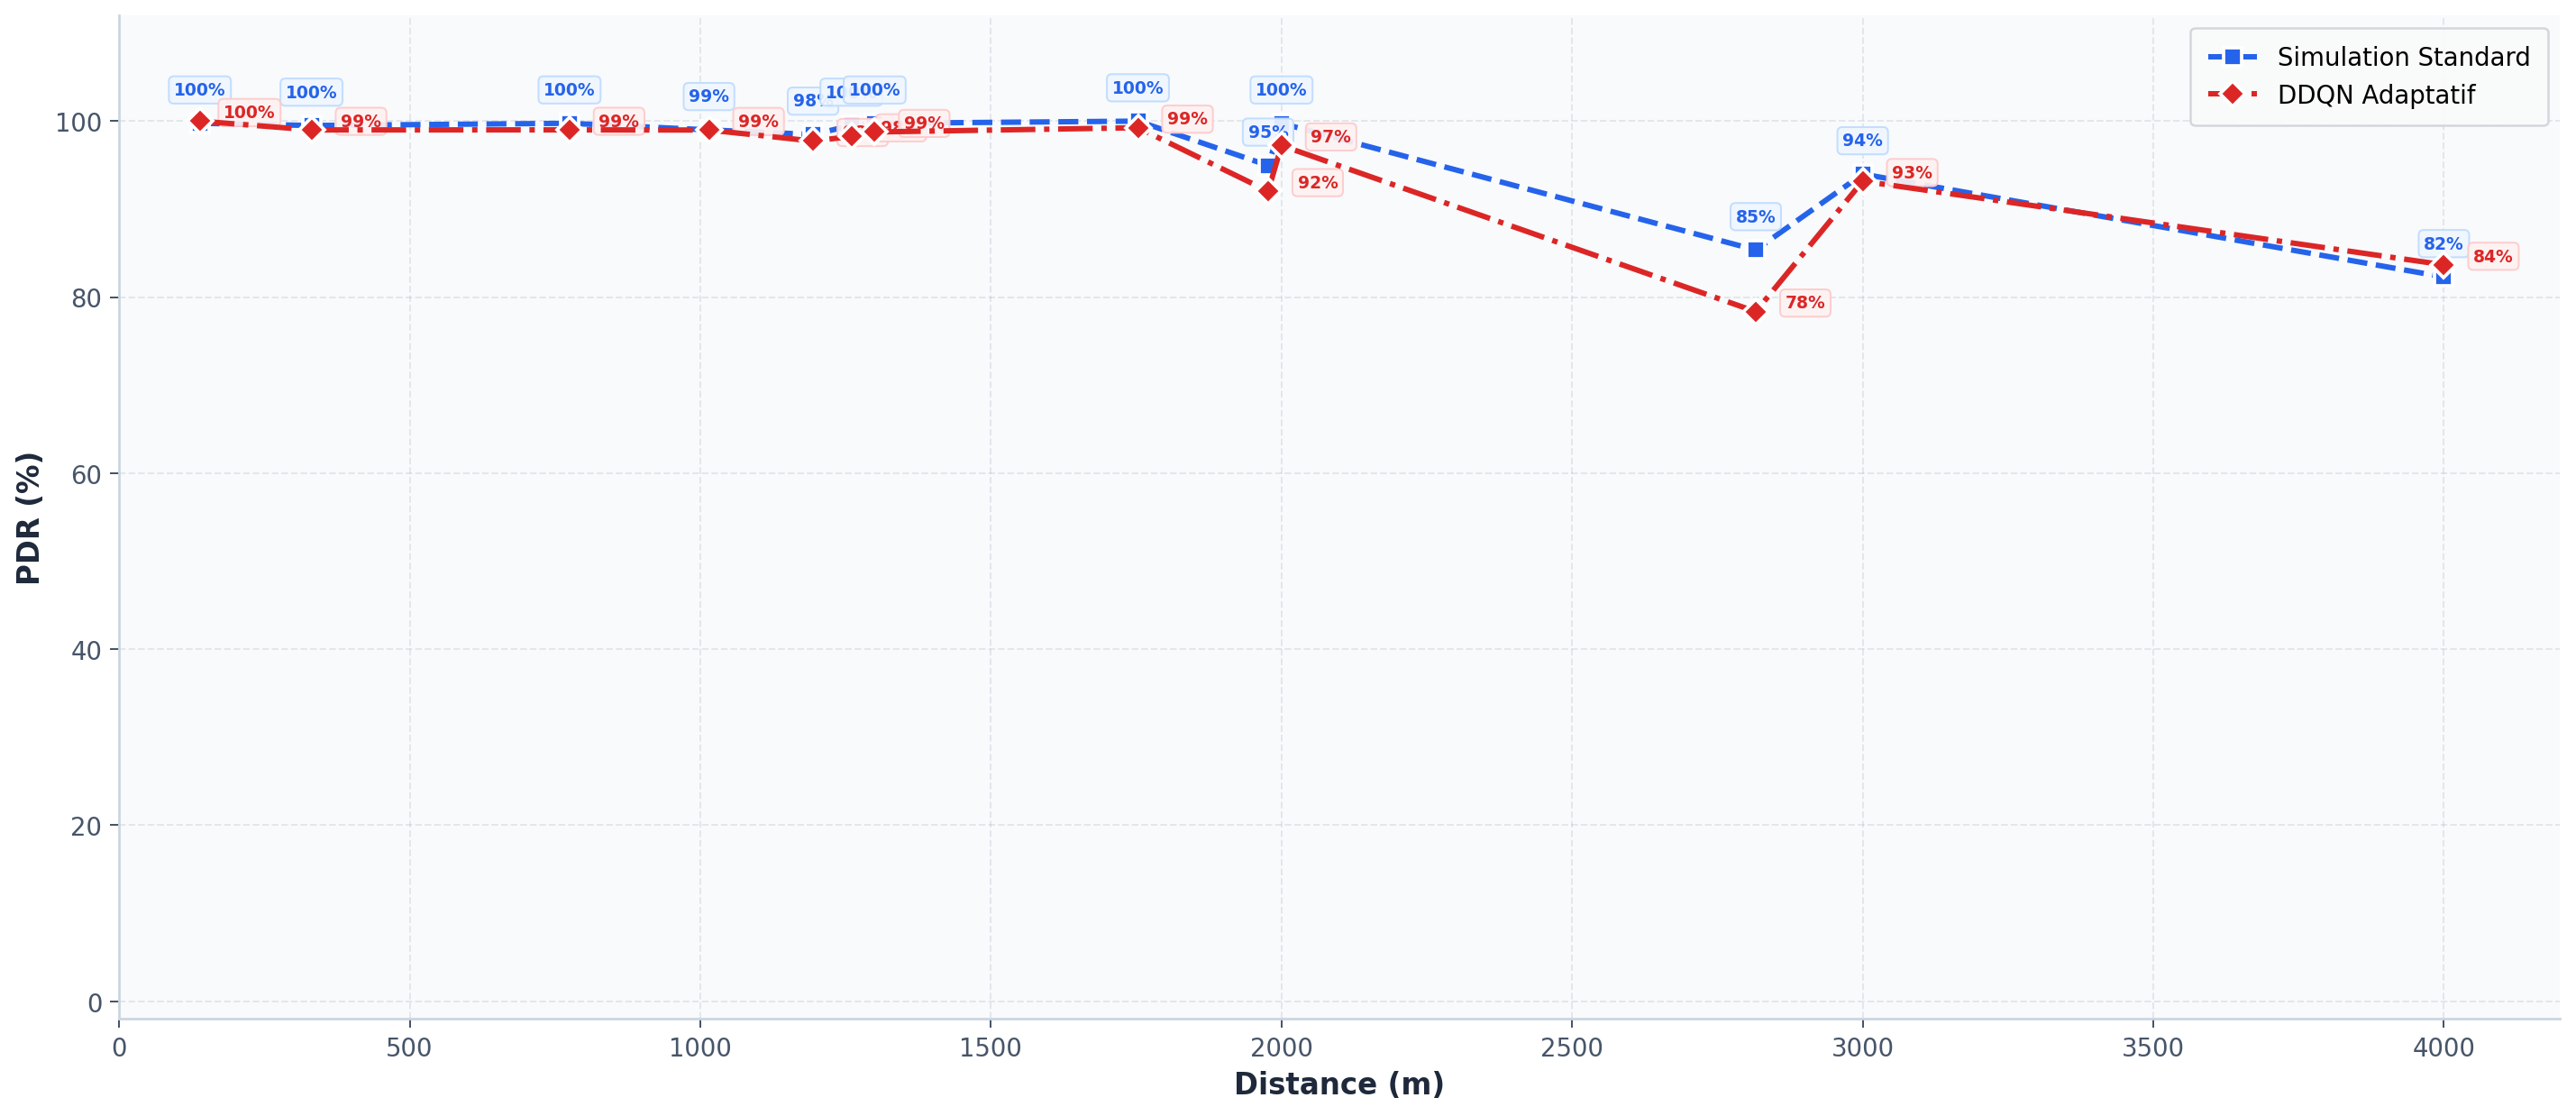
\includegraphics[width=1\textwidth]{images/validation/ddqn/dr/dr8_pdr_courbes.png}
		\caption{Comparaison PDR pour DR8 : Standard vs DDQN}
		\label{fig:dr8-pdr}
	\end{figure}
	
	\begin{figure}[H]
		\centering
		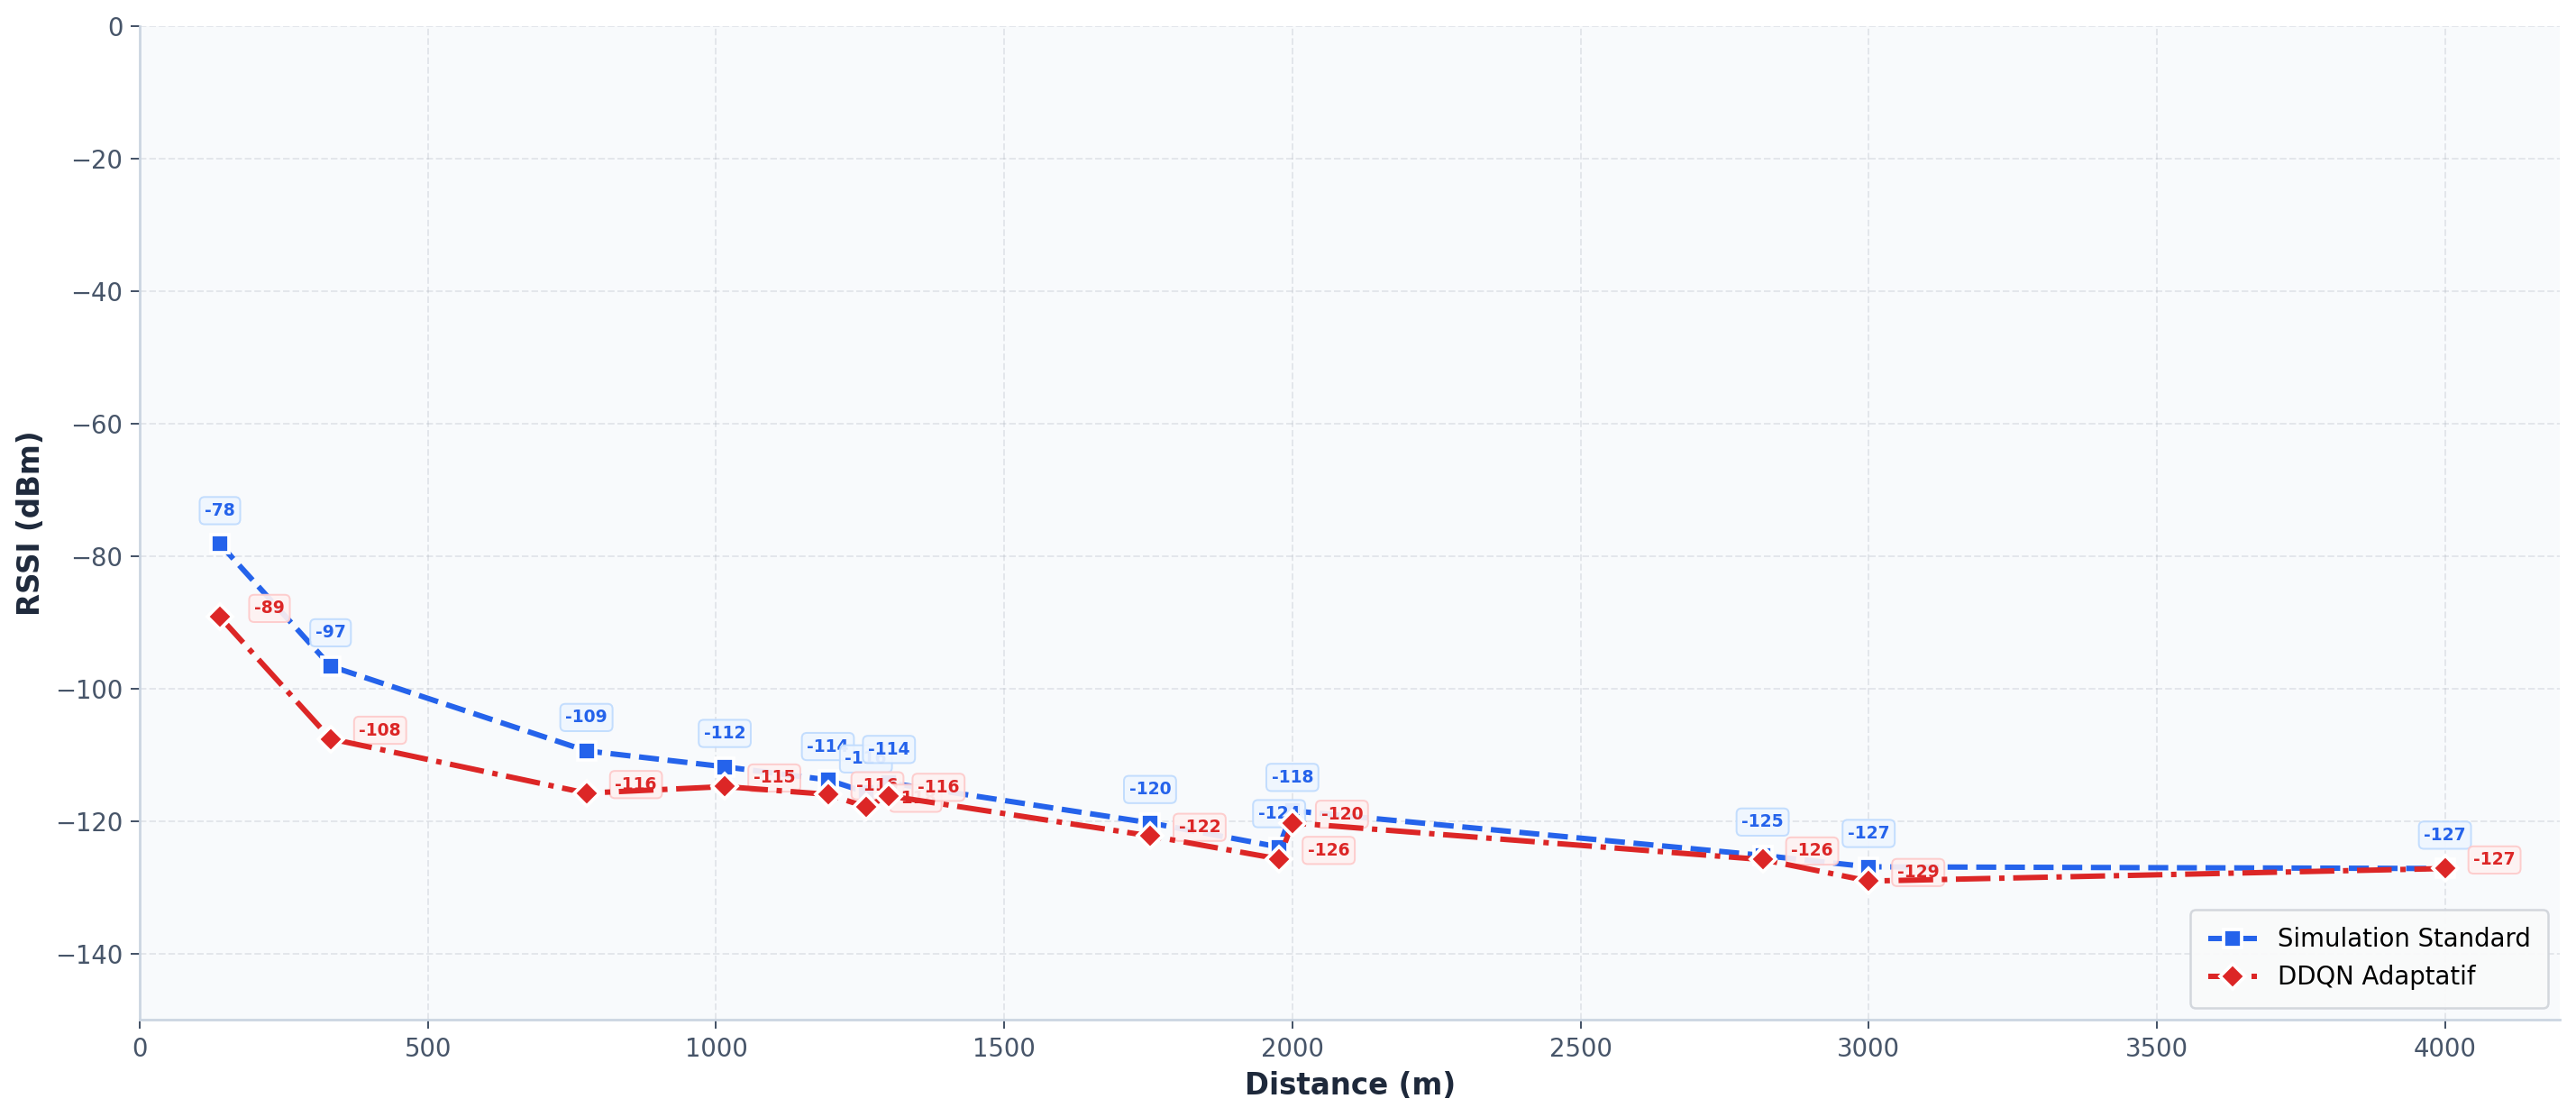
\includegraphics[width=1\textwidth]{images/validation/ddqn/dr/dr8_rssi_courbes.png}
		\caption{Comparaison RSSI pour DR8 : Standard vs DDQN}
		\label{fig:dr8-rssi}
	\end{figure}
	
	Pour le DR8, l'agent DDQN démontre un bon niveau de performance. Grâce à l'utilisation adaptative de différents débits (DR) et niveaux de puissance d'émission, l'agent DDQN parvient à obtenir des résultats comparables à ceux obtenus avec l'utilisation exclusive du DR8 à puissance d'émission maximale de 14 dBm.
	
	\newpage
	\item \textbf{Analyse pour DR9 (CR 2/3, BW 137 kHz)}
	
	\begin{figure}[H]
		\centering
		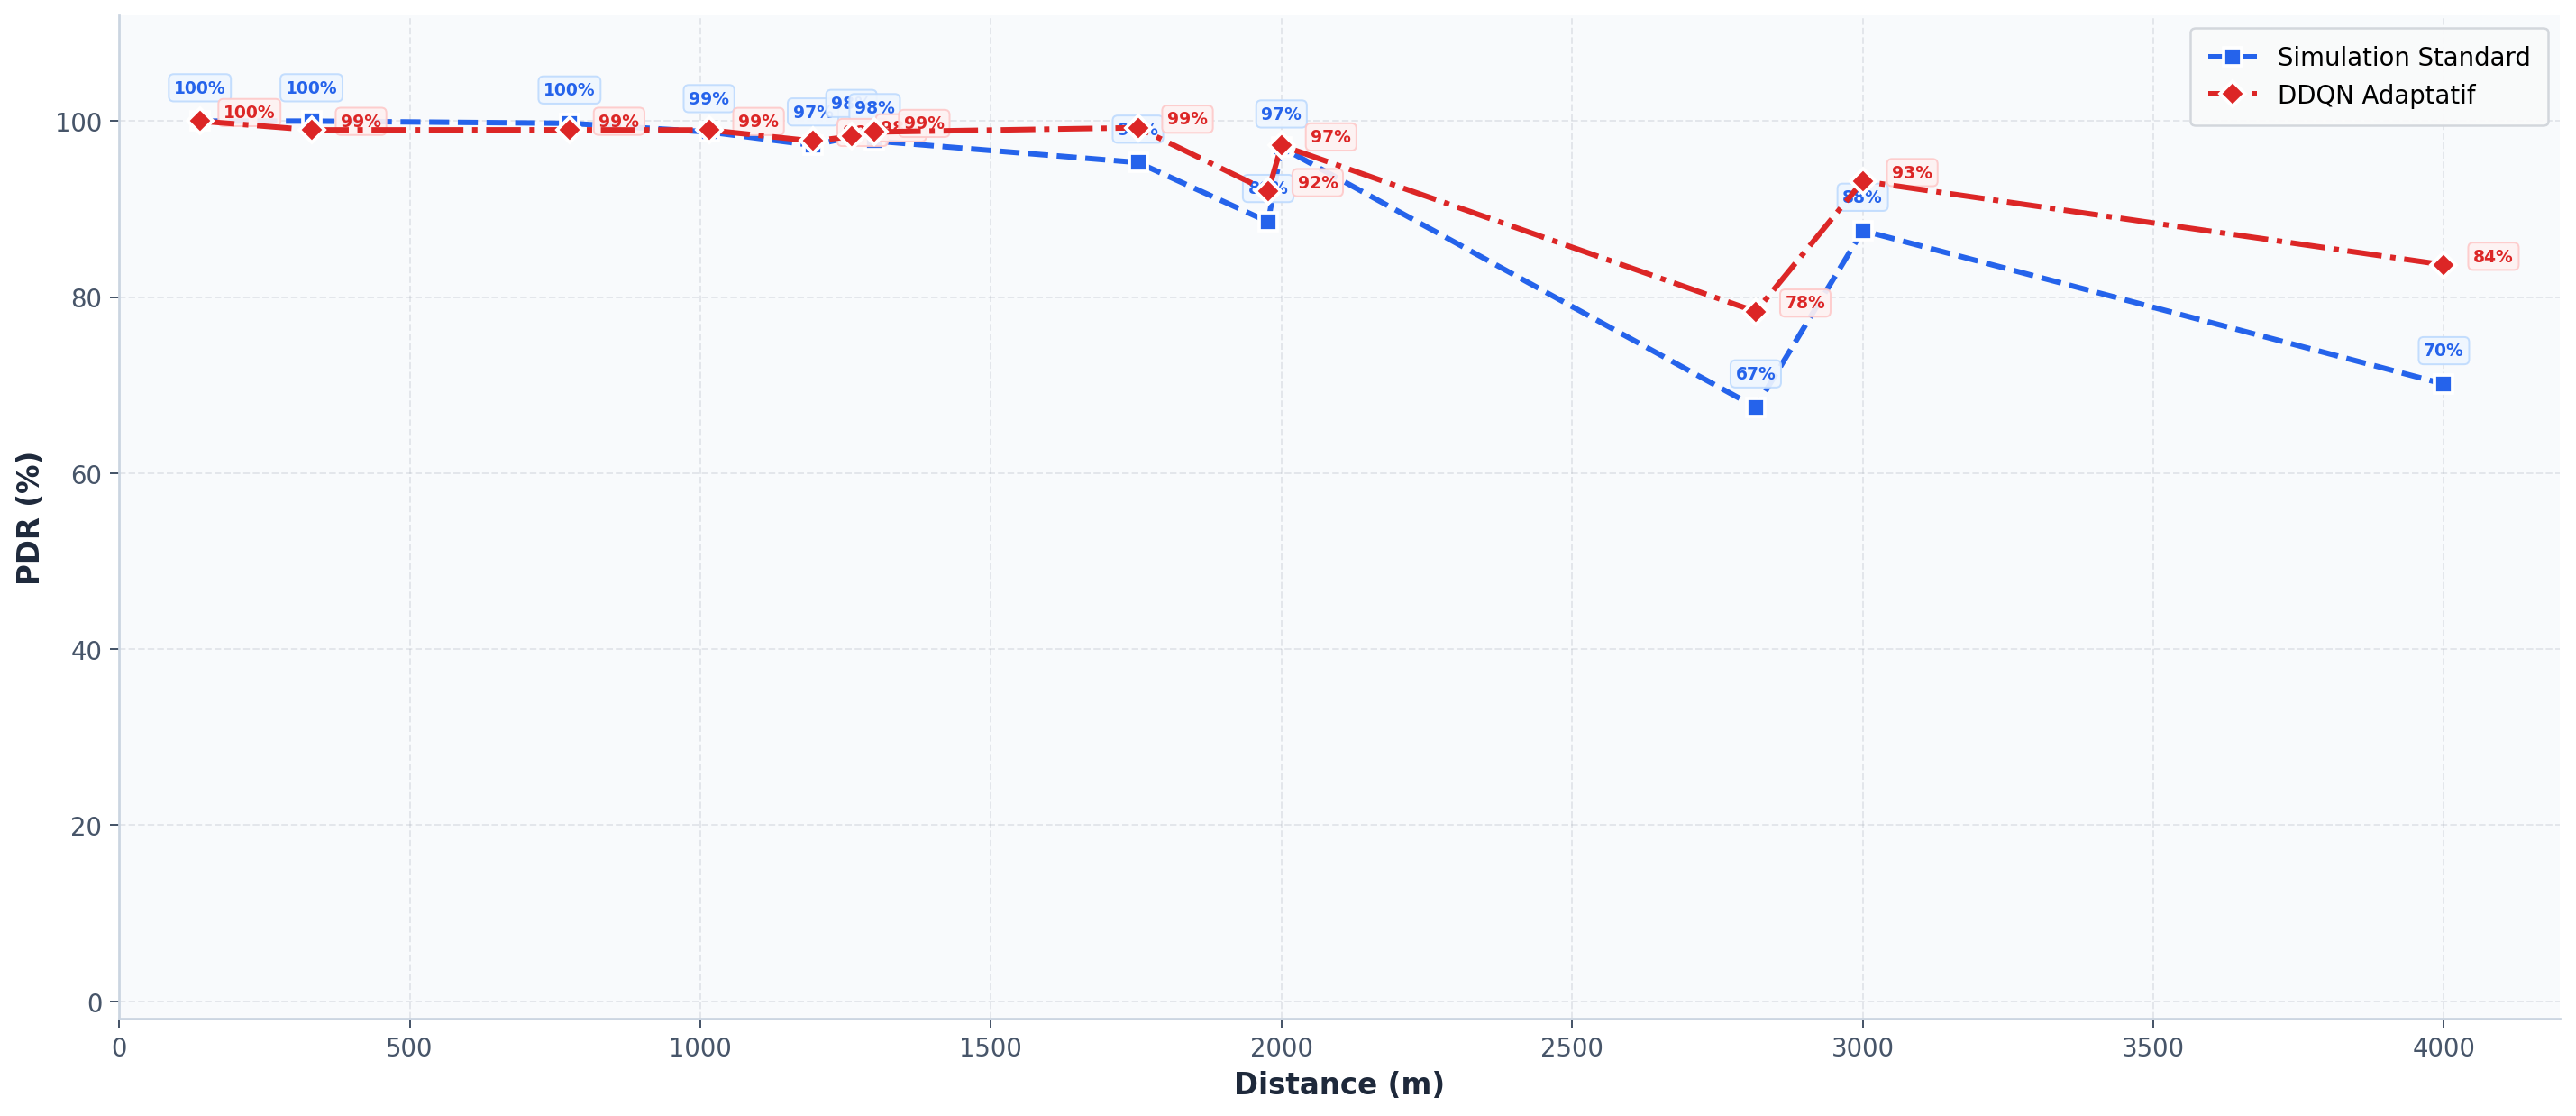
\includegraphics[width=1\textwidth]{images/validation/ddqn/dr/dr9_pdr_courbes.png}
		\caption{Comparaison PDR pour DR9 : Standard vs DDQN}
		\label{fig:dr9-pdr}
	\end{figure}
	
	\begin{figure}[H]
		\centering
		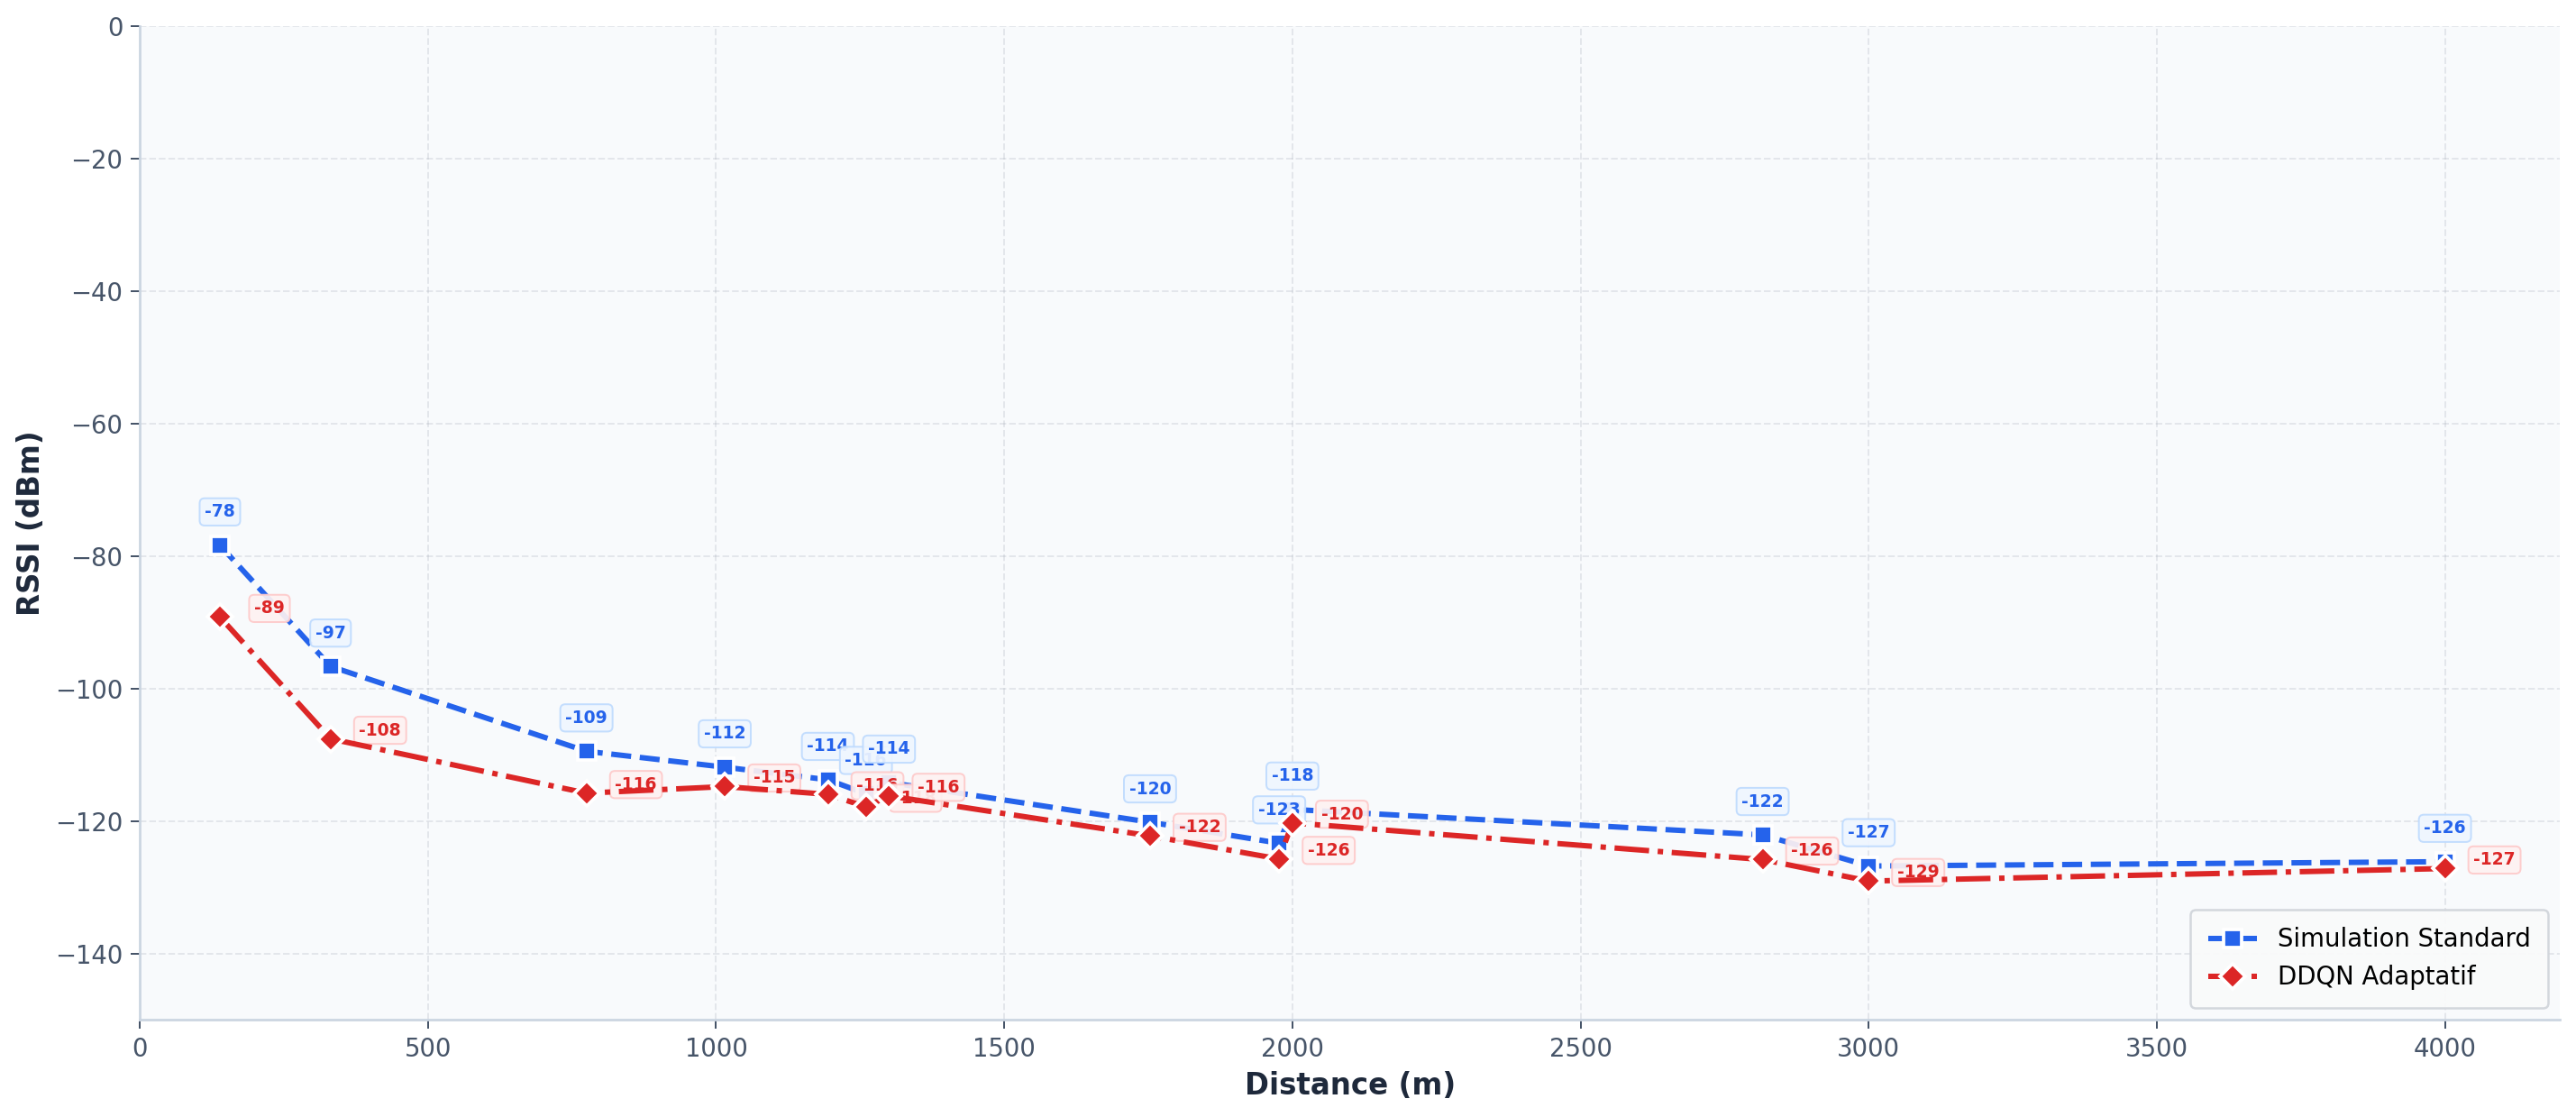
\includegraphics[width=1\textwidth]{images/validation/ddqn/dr/dr9_rssi_courbes.png}
		\caption{Comparaison RSSI pour DR9 : Standard vs DDQN}
		\label{fig:dr9-rssi}
	\end{figure}
	
	Pour le DR9, l'agent DDQN montre une nette supériorité, en particulier aux moyennes et longues distances. Notamment à 4000 m, il atteint un PDR de 84\%, contre 70\% pour la simulation standard, soit un gain absolu de 14 points et une amélioration relative d'environ 20\%.
	
	\newpage
	\item \textbf{Analyse pour DR10 (CR 1/3, BW 336 kHz)}
	
	\begin{figure}[H]
		\centering
		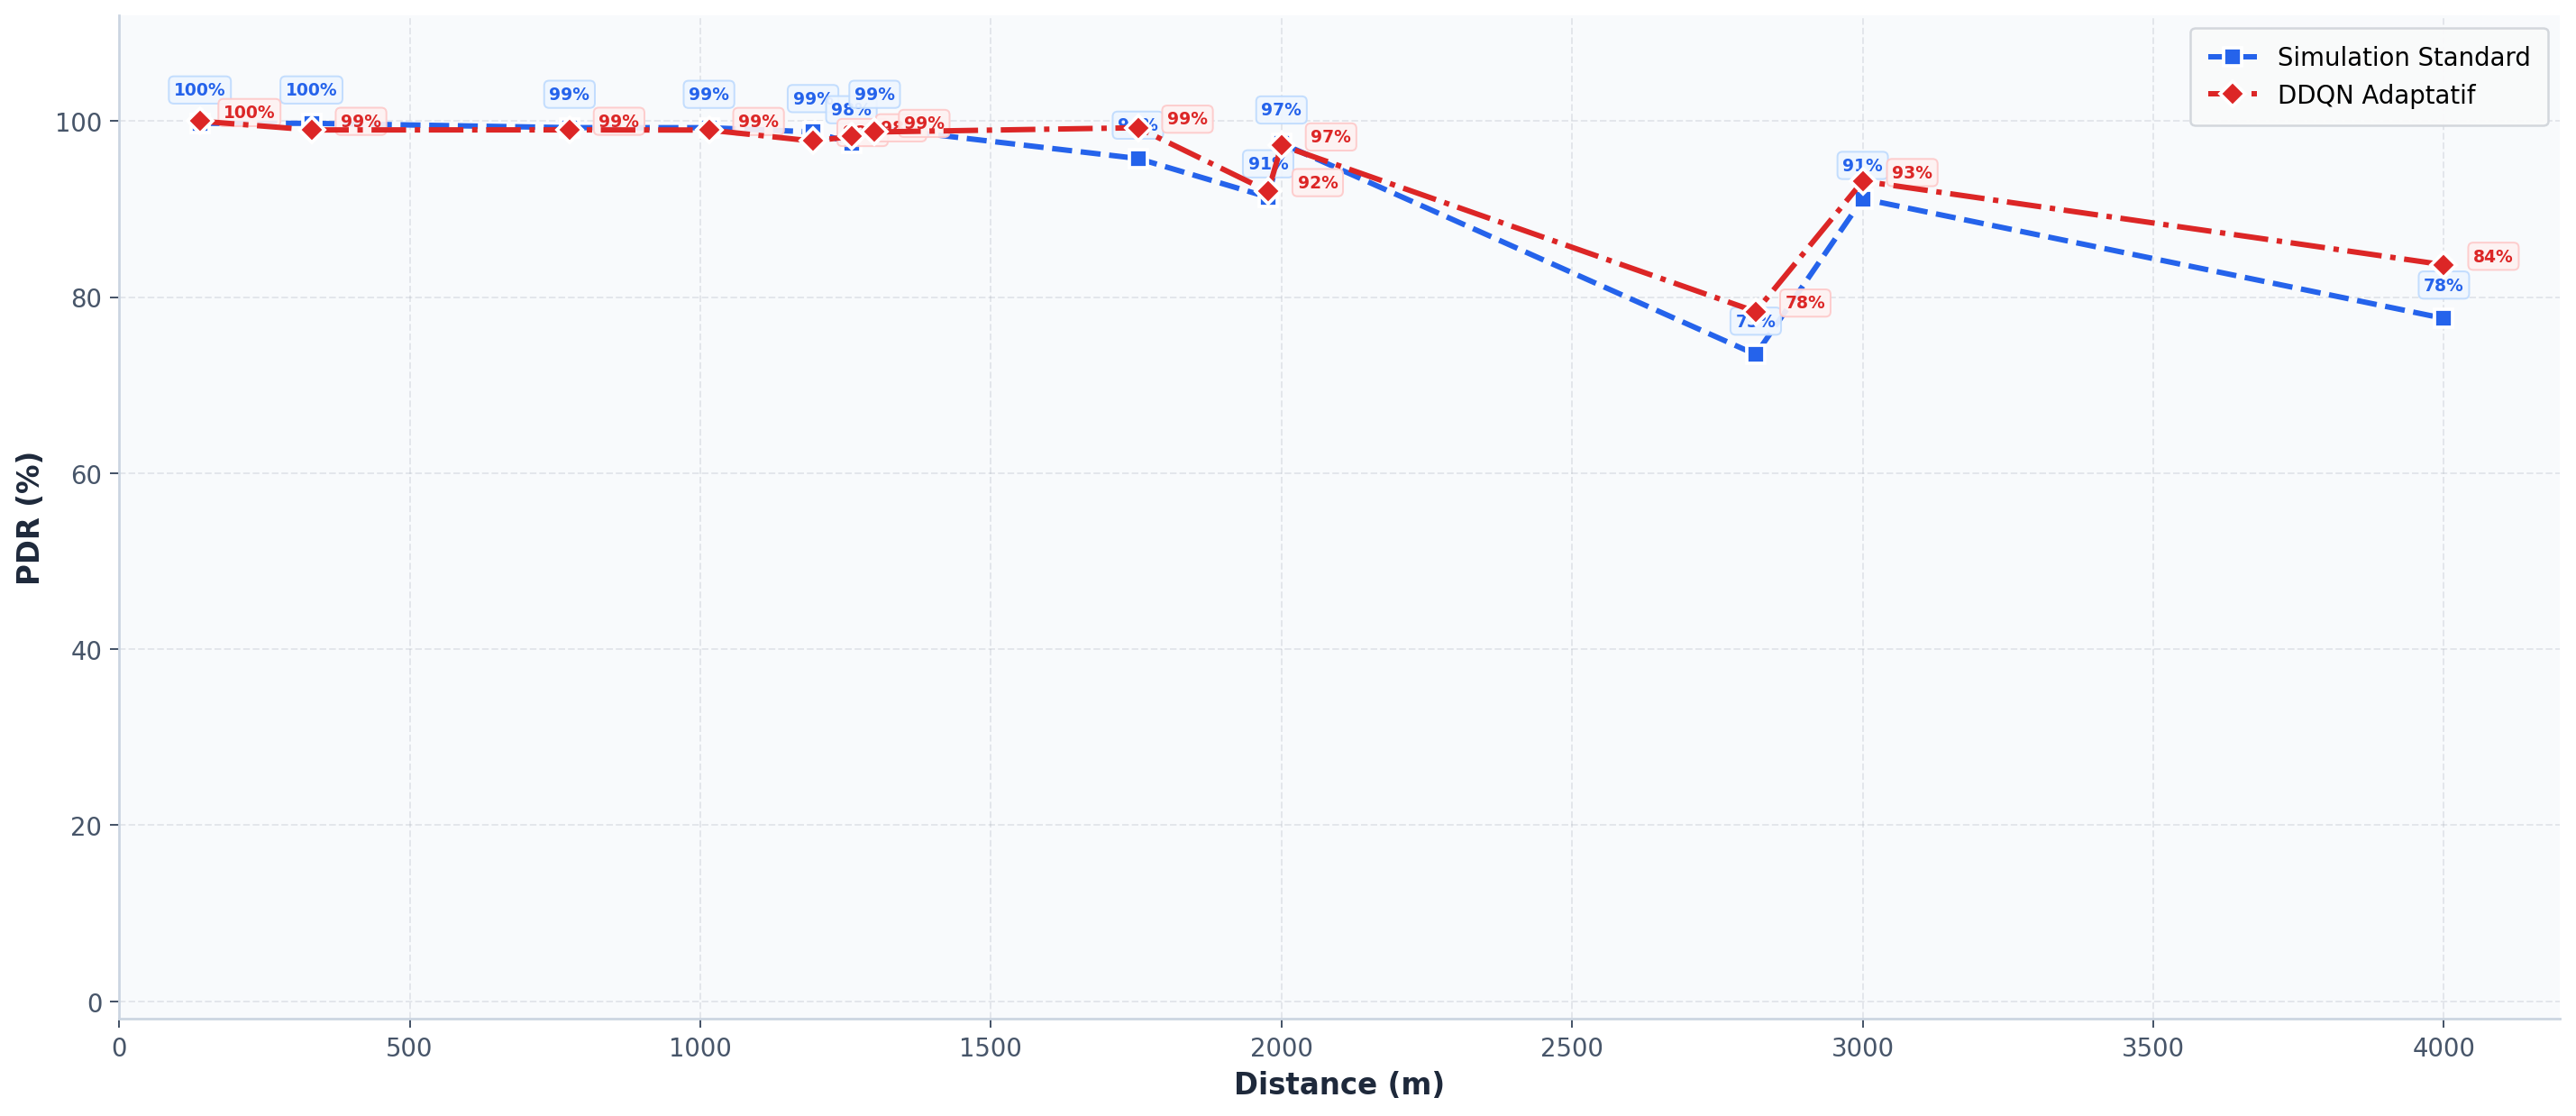
\includegraphics[width=1\textwidth]{images/validation/ddqn/dr/dr10_pdr_courbes.png}
		\caption{Comparaison PDR pour DR10 : Standard vs DDQN}
		\label{fig:dr10-pdr}
	\end{figure}
	
	\begin{figure}[H]
		\centering
		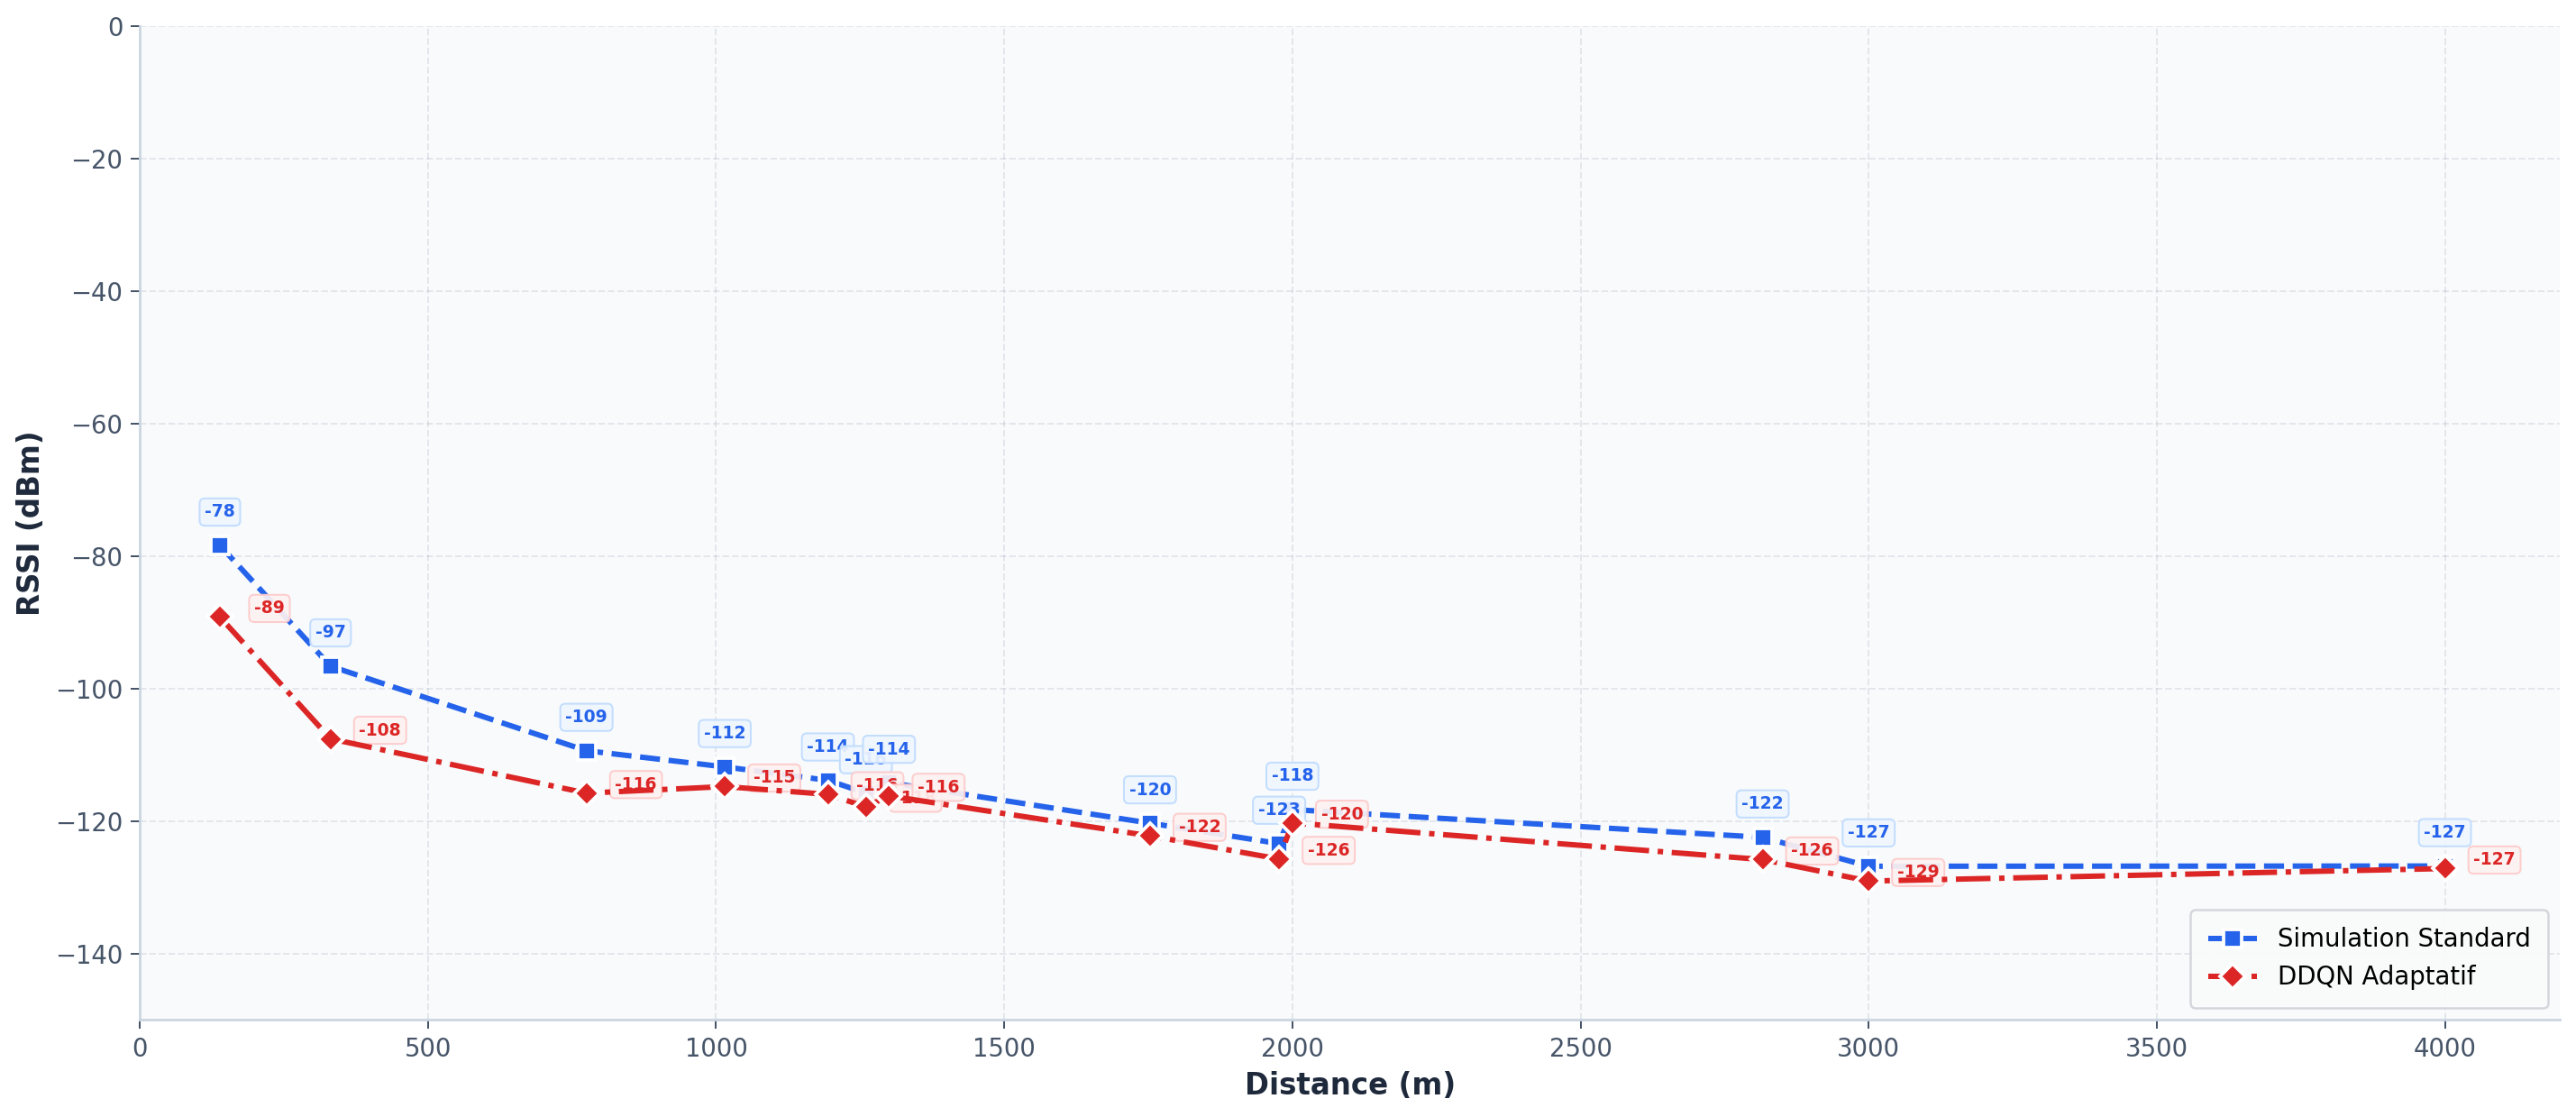
\includegraphics[width=1\textwidth]{images/validation/ddqn/dr/dr10_rssi_courbes.png}
		\caption{Comparaison RSSI pour DR10 : Standard vs DDQN}
		\label{fig:dr10-rssi}
	\end{figure}
	
	Le DDQN se montre également performant pour le DR10, avec un écart plus marqué que celui observé pour le DR8 (\ref{fig:dr8-pdr}). À 4000 m, le PDR atteint 84\% avec le DDQN, contre 78\% pour la simulation standard, soit un gain absolu de 6 points et une amélioration relative d'environ 7,6\%.
	
	\newpage
	\item \textbf{Analyse pour DR11 (CR 2/3, BW 336 kHz)}
	
	\begin{figure}[H]
		\centering
		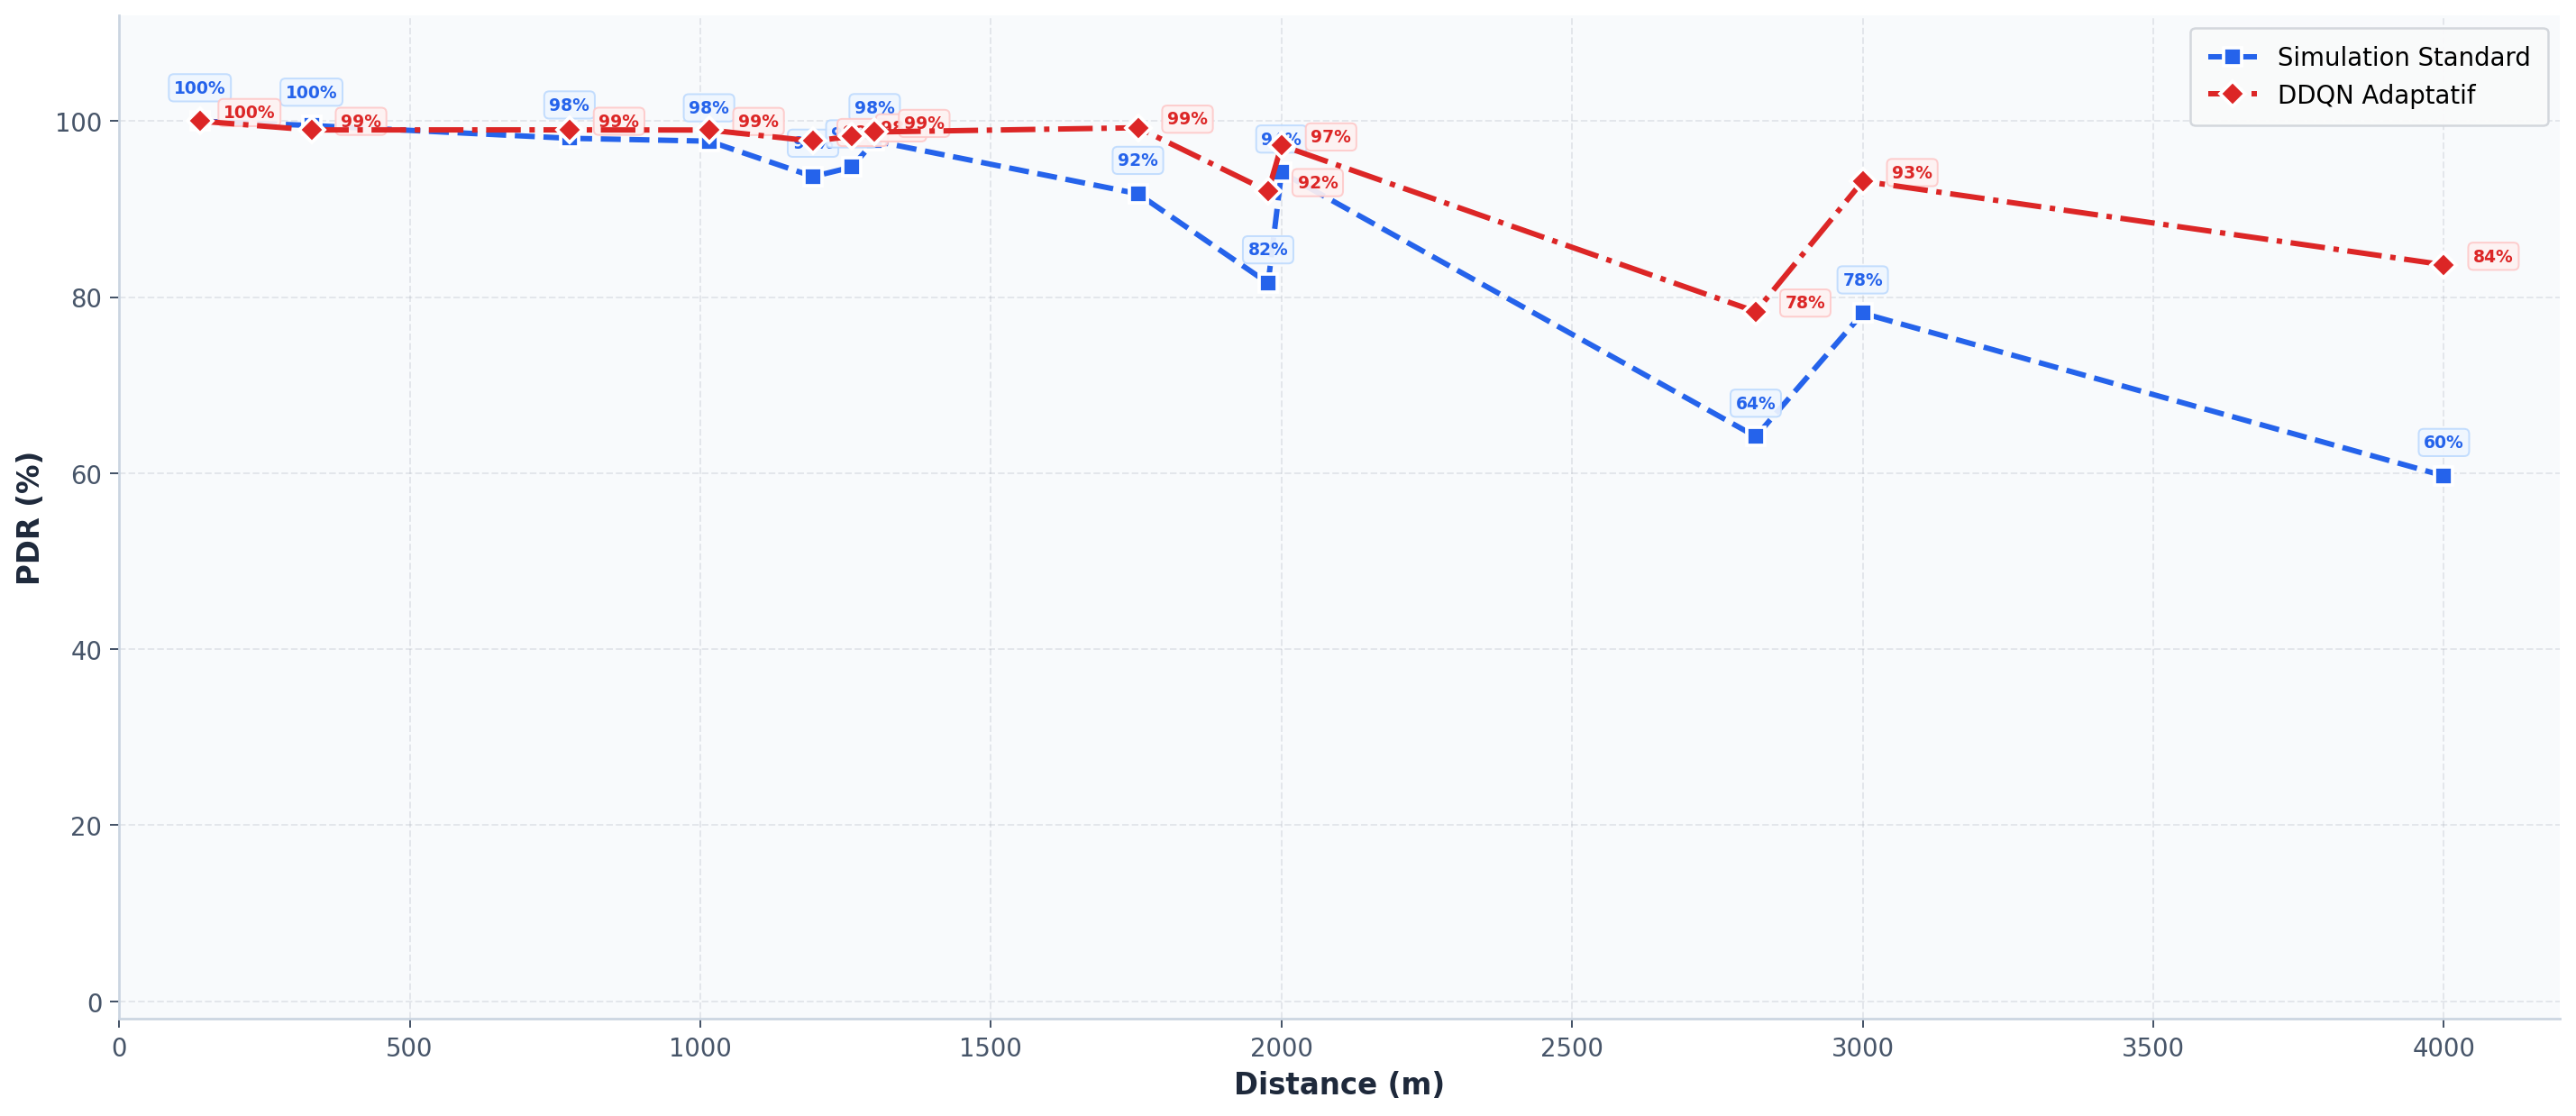
\includegraphics[width=1\textwidth]{images/validation/ddqn/dr/dr11_pdr_courbes.png}
		\caption{Comparaison PDR pour DR11 : Standard vs DDQN}
		\label{fig:dr11-pdr}
	\end{figure}
	
	\begin{figure}[H]
		\centering
		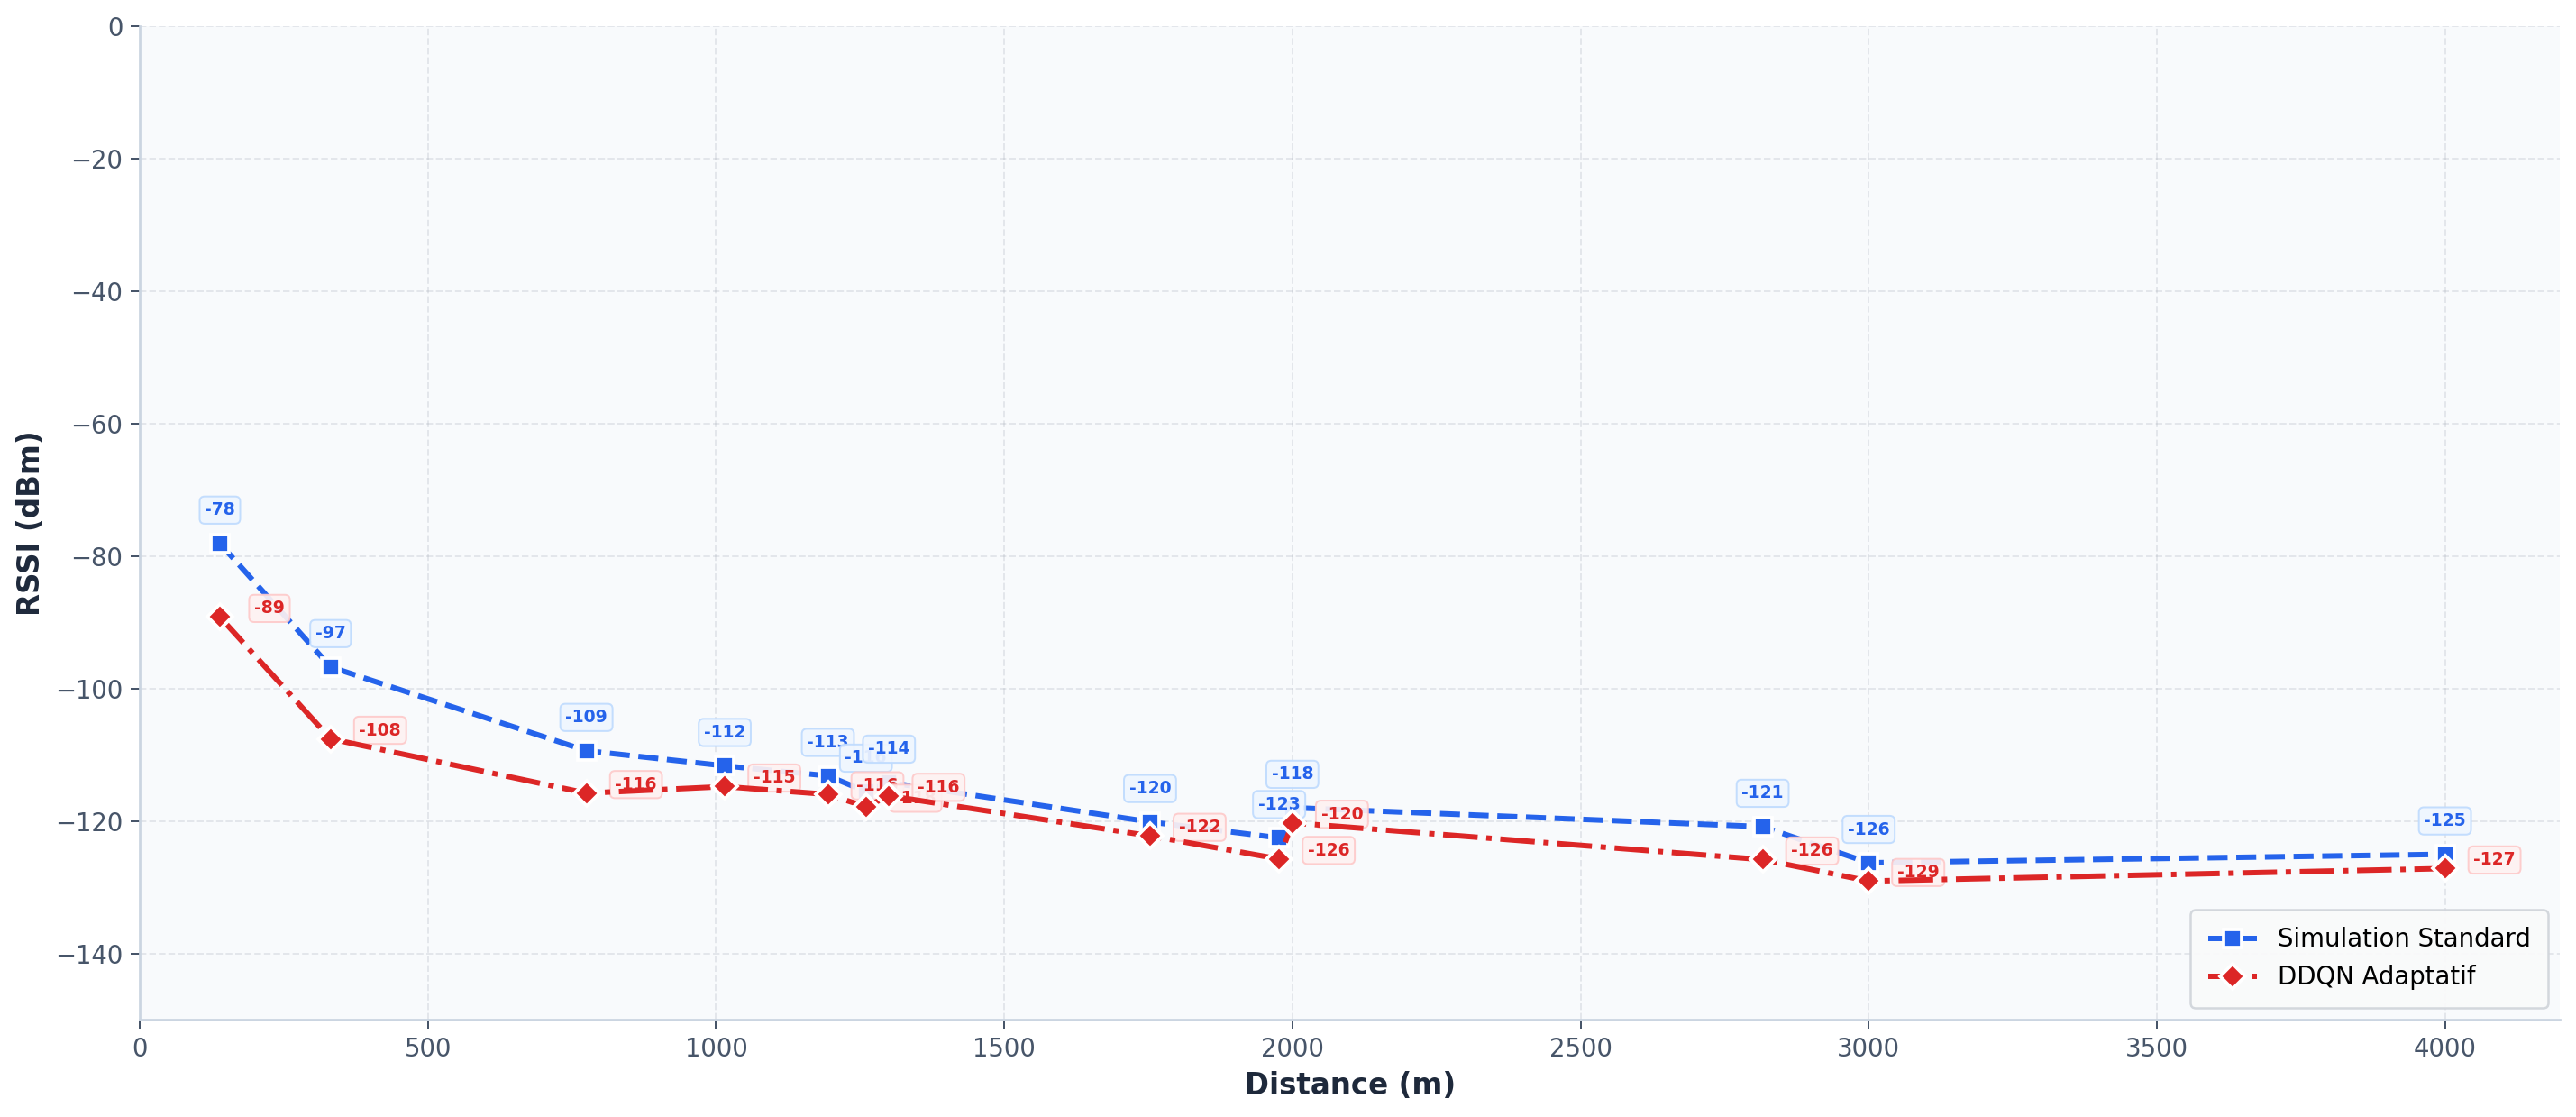
\includegraphics[width=1\textwidth]{images/validation/ddqn/dr/dr11_rssi_courbes.png}
		\caption{Comparaison RSSI pour DR11 : Standard vs DDQN}
		\label{fig:dr11-rssi}
	\end{figure}
	
	Pour le DR11, l'agent DDQN s'impose largement. Au-delà de 1000 m, il présente un taux de succès supérieur à celui du DR11 seul. À 4000 m, le PDR atteint 84\% avec le DDQN, contre 60\% pour le DR11, soit un gain absolu de 24 points et une amélioration relative d'environ 40\%.\\
	\\
	Un comportement similaire est observé concernant l'évolution du RSSI, quel que soit le DR. L'agent DDQN présente un RSSI plus faible sur l'ensemble des distances, avec un effet encore plus marqué sur les courtes distances. Cela illustre sa capacité à adapter dynamiquement la puissance d'émission.
\end{itemize}

\subsection{Analyse des performances par distance}

\begin{itemize}
	\item \textbf{Analyse du PDR}
	
	Le tableau \ref{tab:comparaison-pdr} présente la comparaison détaillée du taux de livraison (PDR) entre la simulation standard et l'agent DDQN pour les 13 distances évaluées. La colonne Standard représente la moyenne des 4 DR statiques.
	
	\begin{table}[H]
		\centering
		\caption{Comparaison du PDR : simulation standard vs agent DDQN}
		\label{tab:comparaison-pdr}
		\begin{tabular}{|c|c|c|c|c|}
			\hline
			\textbf{Distance (m)} & \textbf{Standard (\%)} & \textbf{DDQN (\%)} & \textbf{Variation (pts)} & \textbf{Taux (\%)}\\
			\hline
			\hline
			139  & 99,9 & 100,0 & +0,1 &\cellcolor{green!30} +0,1\\
			\hline
			331  & 99,7 & 99,0  & -0,7 & \cellcolor{red!30} -0,7 \\
			\hline
			775  & 99,2 & 99,0  & -0,2 & \cellcolor{red!30} -0,2\\
			\hline
			1015 & 98,7 & 99,0  & +0,3 &\cellcolor{green!30} +0,3\\
			\hline
			1194 & 97,1 & 97,7  & +0,6 &\cellcolor{green!30} +0,7\\
			\hline
			1260 & 97,5 & 98,3  & +0,8 &\cellcolor{green!30} +0,8\\
			\hline
			1300 & 98,6 & 98,8  & +0,2 & \cellcolor{green!30}+0,2\\
			\hline
			1753 & 95,7 & 99,2  & +3,5 & \cellcolor{green!30}+3,66\\
			\hline
			1977 & 89,1 & 92,0  & +2,9 &\cellcolor{green!30} +3,25\\
			\hline
			2000 & 97,1 & 97,2  & +0,1 &\cellcolor{green!30} +0,1\\
			\hline
			2816 & 72,6 & 78,4  & +5,8 &\cellcolor{green!30} +7,99 \\
			\hline
			3000 & 87,7 & 93,2  & +5,5 &\cellcolor{green!30}+6,27\\
			\hline
			4000 & 72,4 & 83,7  & +11,3 &\cellcolor{green!30} +15,6 \\
			\hline
			\hline
			\textbf{Moyenne} & \textbf{92,7} & \textbf{95,0} & \textbf{+2,3} & \cellcolor{green!30} \textbf{+2,48} \\
			\hline
		\end{tabular}
	\end{table}
	
	L'agent DDQN améliore le PDR dans 11 cas sur 13 (85\% des distances), avec une amélioration moyenne de 2,3 points. Les gains les plus significatifs sont observés aux longues distances : +11,3 points à 4000 m, +5,8 points à 2816 m et +5,5 points à 3000 m.
	
	\item \textbf{Analyse du débit}
	
	Le tableau suivant présente l'évolution du débit moyen de l'agent DDQN comparé au débit moyen bas (DR8/DR10) et haut (DR9/DR11) dans les mêmes conditions.
	
	\begin{table}[H]
		\centering
		\caption{Évolution du débit en fonction de la distance}
		\label{tab:debit_distance}
		\begin{tabular}{|c|c|c|c|c|}
			\hline
			\textbf{Distance (m)} &  \textbf{DR8/10 (bps)} & \textbf{DR9/11 (bps)} &   \textbf{Moyenne (bps)} & \textbf{DDQN (bps)} \\
			\hline
			139    & 89,59  & 142,05 & 115,82 & 142,05 \\
			\hline
			331    & 89,59  & 142,05 & 115,82 & 140,73 \\
			\hline
			775    & 89,59  & 142,05 & 115,82 & 90,11 \\
			\hline
			1015-4000 & 89,59  & 142,05 & 115,82  & 89,59 \\
			\hline
		\end{tabular}
	\end{table}
	Pour maximiser la fiabilité à longue distance, l'agent DDQN sacrifie le débit de manière délibérée, en privilégiant systématiquement les configurations les plus robustes (DR8/10).
		
	\item \textbf{Analyse de la puissance d'émission}
	
	Le tableau suivant présente l'évolution de la puissance de transmission utilisée par l'agent DDQN en fonction de la distance, comparativement à la puissance fixe de l'approche standard.
	
	\begin{table}[H]
		\centering
		\caption{Comparaison de la puissance d'émission}
		\label{tab:comparaison-puissance}
		\begin{tabular}{|c|c|c|c|}
			\hline
			\textbf{Distance (m)} & \textbf{Puiss. Standard (dBm)} & \textbf{Puiss. DDQN (dBm)} & \textbf{Réduction (\%)} \\
			\hline
			\hline
			139  & 14,0 & 3,0  & 78,6 \% \\
			\hline
			331  & 14,0 & 3,1  & 77,9 \% \\
			\hline
			775  & 14,0 & 7,6  & 45,7 \% \\
			\hline
			1015 & 14,0 & 11,1 & 20,7 \% \\
			\hline
			1194 & 14,0 & 11,9 & 15,0 \% \\
			\hline
			1260 & 14,0 & 12,0 & 14,3 \% \\
			\hline
			1300 & 14,0 & 12,0 & 14,3 \% \\
			\hline
			1753 & 14,0 & 12,0 & 14,3 \% \\
			\hline
			1977 & 14,0 & 12,0 & 14,3 \% \\
			\hline
			2000 & 14,0 & 12,0 & 14,3 \% \\
			\hline
			2816 & 14,0 & 12,0 & 14,3 \% \\
			\hline
			3000 & 14,0 & 12,0 & 14,3 \% \\
			\hline
			4000 & 14,0 & 14,0 & 0,0 \% \\
			\hline
			\hline
			\textbf{Moyenne} & \textbf{14,0} & \textbf{9,5} & \textbf{32,0 \%} \\
			\hline
		\end{tabular}
	\end{table}
	
	L'analyse de la puissance d'émission révèle une réduction moyenne de 32\%, avec des économies importantes aux courtes distances (jusqu'à 78,6\% à 139 m). Cette réduction de puissance contribue directement à l'efficacité énergétique globale du système.
	
	\newpage
	\item \textbf{Comparaison énergétique}
	
	Le tableau suivant présente la consommation énergétique de l'approche standard et de l'agent DDQN.
	
	\begin{table}[H]
		\centering
		\caption{Comparaison de l'énergie consommée par paquet}
		\label{tab:comparaison-energie}
		\begin{tabular}{|c|c|c|c|}
			\hline
			\textbf{Distance (m)} & \textbf{Énergie Std (mJ)} & \textbf{Énergie DDQN (mJ)} & \textbf{Variation (\%)} \\
			\hline
			\hline
			139  & 76,88 & 28,81  & \cellcolor{green!30} -62,5 \% \\
			\hline
			331  & 76,92 & 29,62  & \cellcolor{green!30} -61,5 \% \\
			\hline
			775  & 76,95 & 61,65  & \cellcolor{green!30} -19,9 \% \\
			\hline
			1015 & 76,91 & 77,14  & \cellcolor{red!30} +0,3 \% \\
			\hline
			1194 & 76,95 & 81,73  &\cellcolor{red!30} +6,2 \% \\
			\hline
			1260 & 76,98 & 82,51  &\cellcolor{red!30} +7,2 \% \\
			\hline
			1300 & 76,93 & 82,51  &\cellcolor{red!30} +7,3 \% \\
			\hline
			1753 & 76,86 & 82,51  &\cellcolor{red!30} +7,3 \% \\
			\hline
			1977 & 76,86 & 82,51  & \cellcolor{red!30}+7,3 \% \\
			\hline
			2000 & 76,88 & 82,51  & \cellcolor{red!30}+7,3 \% \\
			\hline
			2816 & 76,85 & 82,51  &\cellcolor{red!30} +7,4 \% \\
			\hline
			3000 & 77,00 & 82,54  & \cellcolor{red!30}+7,2 \% \\
			\hline
			4000 & 77,05 & 94,29  &\cellcolor{red!30} +22,4 \% \\
			\hline
			\hline
			\textbf{Moyenne} & \textbf{76,93} & \textbf{73,14} & \cellcolor{green!30} \textbf{-4,9 \%} \\
			\hline
		\end{tabular}
	\end{table}
	
	La consommation énergétique par paquet est réduite de 4,9\% en moyenne, avec des économies substantielles aux courtes distances, atteignant 62,5\% à 139 m. Aux distances intermédiaires, un léger surcoût de l'ordre de 6 à 7\% est observé, mais celui-ci est largement compensé par les gains de fiabilité obtenus sur le PDR.
	À 4000 m, le surcoût de 22,4\% s'explique par la nature même de la référence de comparaison. En effet, la simulation standard représente la moyenne des quatre DR statiques (DR8, DR9, DR10, DR11), tous émis à la puissance maximale de 14 dBm. Or, les configurations DR9 et DR11 (CR = 2/3) génèrent un temps d'antenne structurellement plus court que DR8 et DR10 (CR = 1/3), ce qui abaisse considérablement la consommation énergétique moyenne de référence. À l'inverse, l'agent DDQN, face à la dégradation du canal à longue distance, bascule délibérément vers les configurations les plus robustes (DR8/DR10, CR = 1/3), dont le temps d'antenne plus long entraîne une consommation par paquet plus élevée. Ce surcoût énergétique constitue donc un arbitrage intentionnel : il permet un gain de PDR de 11,3 points à 4000 m, soit une amélioration relative de 15,6\%, ce qui confirme la pertinence de la stratégie adoptée par l'agent dans les conditions de canal les plus défavorables.
	
\end{itemize}

\newpage
\subsection{Synthèse des gains apportés par le DDQN}

Ce tableau présente les apports de l'agent DDQN sur les plages de distance.

\begin{table}[H]
	\centering
	\caption{Synthèse des performances par plage de distance}
	\label{tab:synthese-plages}
	\begin{tabular}{|l|c|c|c|c|}
		\hline
		\textbf{Plage de distance} & \textbf{Cas} & \textbf{PDR (pts)} & \textbf{Puissance (dBm)} & \textbf{Énergie (\%)} \\
		\hline
		\hline
		Courte (< 1000 m)      & 3  & \cellcolor{red!30}-0,3 & \cellcolor{green!30}-9,4 & \cellcolor{green!30} -47,9 \% \\
		\hline
		Moyenne (1000-2000 m)  & 7  & \cellcolor{green!30} +1,1 & \cellcolor{green!30}-2,1 &\cellcolor{red!30} +6,1 \% \\
		\hline
		Longue (> 2000 m)      & 3  & \cellcolor{green!30}+7,5 & \cellcolor{green!30}-1,5 & \cellcolor{red!30}+12,3 \% \\
		\hline
	\end{tabular}
\end{table}

Cette analyse par plage de distance révèle la stratégie adaptative optimale de l'agent DDQN :
\begin{itemize}
	\item \textbf{Courtes distances} : Économies d'énergie massives sans compromis sur la fiabilité
	\item \textbf{Distances moyennes} : Investissement énergétique modéré pour un gain de PDR significatif
	\item \textbf{Longues distances} : Forte amélioration de la fiabilité pour un surcoût énergétique acceptable
\end{itemize}

Le tableau \ref{tab:synthese-gains} synthétise les gains quantitatifs apportés par notre solution, avec une moyenne globale sur toutes les distances.

\begin{table}[H]
	\centering
	\caption{Synthèse globale des gains apportés par l'agent DDQN}
	\label{tab:synthese-gains}
	\begin{tabular}{|l|c|c|c|}
		\hline
		\textbf{Métrique} & \textbf{Standard} & \textbf{DDQN} & \textbf{Gain} \\
		\hline
		\hline
		PDR moyen (\%) & 92,7 & 95,0 & \textbf{+2,48\%} \\
		\hline
		Puissance moyenne (dBm) & 14,0 & 9,5 & \textbf{-32,14 \%} \\
		\hline
		Énergie moyenne par paquet (mJ) & 76,93 & 73,14 & \textbf{-4,9 \%} \\
		\hline
		Énergie minimale (mJ) & 76,88 & 28,81 & \textbf{-62,5 \%} \\
		\hline
		PDR à 4000 m (\%) & 72,4 & 83,7 & \textbf{+15,6\%} \\
		\hline
		Cas favorables (PDR) & 2/13 & 11/13 & \textbf{84,61 \%} \\
		\hline
	\end{tabular}
\end{table}

Ces gains s'expliquent par ces mécanismes clés :
\begin{enumerate}
	\item \textbf{Évitement du surdimensionnement} : Ajustement fin de la puissance avec des réductions jusqu'à 78,6\%
	\item \textbf{Sélection adaptative du DR} : Basculement progressif des DR à haut débit vers les DR robustes
\end{enumerate}

\section{Limites et perspectives}

\subsection{Limites de notre solution}

Bien que notre approche ait démontré son efficacité en termes de fiabilité, d'adaptativité et d'économies d'énergie, plusieurs limites doivent être soulignées :

\begin{itemize}
	\item \textbf{Modèle de canal simplifié.} Le modèle de propagation utilisé repose sur une approche \textit{log-distance} avec un ombrage (\textit{shadowing}). Bien que validé par des données terrain récentes \cite{lrfhss_comparaison}, ce modèle ne capture pas les variations temporelles rapides du canal (évanouissements multi-trajets, interférences dynamiques) ni les conditions environnementales changeantes (météo, obstacles mobiles). En conséquence, la fidélité du simulateur pourrait être réduite dans des scénarios plus complexes.
	
	\item \textbf{Agent DDQN entraîné hors ligne.} L’agent a été entraîné dans un environnement à très faible densité, puis ses poids ont été sauvegardés pour la phase d'évaluation. Par conséquent, son comportement face à un trafic réseau plus dense reste à déterminer. De plus, l'apprentissage hors ligne ne permet pas à l'agent de s'adapter en temps réel à des changements imprévus de l'environnement.
	
	\item \textbf{Modèle énergétique partiel.} Notre estimation de la consommation énergétique se limite à l'énergie d'émission, calculée à partir de la puissance de transmission et du temps d'antenne. Elle n'inclut pas la consommation liée à la réception, ni aux échanges protocolaires. L'énergie réelle par paquet utile est donc sous-estimée. De plus, notre évaluation ne mesure pas l'impact énergétique des échecs de transmission (et des retransmissions associées) sur le budget global du nœud.
	
	\item \textbf{Généralisation limitée.} Notre étude s'est concentrée sur un environnement unique (d'après les données de validation), une taille de la charge utile fixe de 1 octet et des nœuds statiques. La validité de nos conclusions dans d'autres contextes (charge utiles longues, mobilité) reste à démontrer.
\end{itemize}



\subsection{Perspectives}

Les limites identifiées précédemment ouvrent naturellement plusieurs axes d'amélioration et extensions pour des travaux futurs :

\begin{itemize}
	\item \textbf{Modélisation plus fine du canal.} Une première perspective consisterait à enrichir le modèle de propagation en intégrant des variations temporelles de l'évanouissement lent (\textit{shadowing}) ou des modèles d'évanouissement plus réalistes (Rice, Nakagami). L'ajout d'un modèle d'interférences permettrait également de simuler des environnements avec plus de réalisme.
	
	\item \textbf{Agent adaptatif et apprentissage en ligne.} L'agent DDQN gagnerait à être évalué dans des conditions plus variées : topologies aléatoires multiples, trafic variable, présence d'autres technologies (LoRa classique). Une évolution majeure serait le passage à un apprentissage en ligne (\textit{online learning}) permettant à l'agent d'ajuster sa politique en temps réel face à des changements environnementaux. L'exploration d'autres architectures d'apprentissage pourrait également être envisagée.
	
	\item \textbf{Modèle énergétique complet :} Une amélioration significative consisterait à développer un modèle énergétique plus exhaustif, conforme à la spécification LoRaWAN classe A. Celui-ci intégrerait la consommation en mode réception (écoute du canal), les échanges d'acquittements, l'énergie de réveil et d'échange protocolaire. Cette extension permettrait d'estimer plus précisément la durée de vie des nœuds et de valider les gains énergétiques annoncés.
	
	\item \textbf{Validation multi-environnements.} Une perspective importante serait de valider notre approche sur plusieurs jeux de données correspondant à des environnements variés (urbain, rural, industriel, intérieur) et des conditions météorologiques différentes. Des campagnes de mesures dédiées, avec des charges utiles réalistes (10 à 50 octets) et des scénarios de mobilité, constitueraient une validation terrain plus impactante.
	
	\item \textbf{Passage à l'échelle et déploiement réel.} Enfin, le comportement de l'agent dans des réseaux de grande taille (plusieurs centaines de nœuds) reste à étudier, notamment en termes de complexité computationnelle et d'adaptation aux interférences. À plus long terme, une implémentation sur plateforme réelle (carte LoRaWAN, gateway) permettrait de valider expérimentalement les gains observés en simulation et d'étudier les défis pratiques liés au déploiement de l'algorithme d'apprentissage.
	
\end{itemize}



\section{Conclusion}

Ce chapitre a présenté une évaluation approfondie de l'agent DDQN pour l'optimisation des transmissions LR-FHSS. En confrontant ses performances à celles de la simulation standard sans DDQN sur un ensemble de distances, nous avons démontré des gains significatifs sur tous les axes de performance, à savoir la fiabilité, l'efficacité énergétique et l'adaptabilité. Nous avons également exposé les limites de notre approche et donné les futures directions d'amélioration.